\Chapter{Problem układania planu lekcji i algorytm jego rozwiązania}\label{chapter:algorytm}
    Opis struktury rozdziału.
    % Chociaż czyste podejście MIP prowadzi do teoretycznie optymalnych rozwiązań, w praktyce jego zastosowanie do pełnego problemu jest niemożliwe.
    % Złożoność obliczeniowa i pamięciowa przekracza możliwości przeciętnych komputerów, co uniemożliwia efektywny rozwój takiego rozwiązania.
    % Ponadto takie rozwiązanie jest też trudne do zaprogramowania ze względu na bloki lekcyjne.

    % Zaprezentowane podejście hybrydowe pozwala pokonać problem złożoności obliczeniowej, oferując praktyczny kompromis między optymalnością a czasem obliczeń.

    \section{Sformułowanie problemu optymalizacyjnego}
        Na potrzeby pracy warto ujednolicić terminologię, z uwagi na to, że w języku potocznym niektóre z tych terminów są używane zamiennie:
        \begin{itemize}
            \item \textbf{Klasa}: Grupa uczniów; przykładowo ,,IIA'', ,,IVC'', \dots
            Ze względu na angielską nazwę \textit{class}, która koliduje ze składnią języków programowania, w kodzie często odnoszę się do klas jako \verb|student_group|.
            \item \textbf{Sala}: Miejsce, w którym prowadzone są zajęcia; przykładowo ,,Sala Gimnastyczna 1'', ,,2'', \dots
            \item \textbf{Przedmiot}: Temat zajęć prowadzonych przez nauczyciela; przykładowo ,,Wychowanie Fizyczne'', ,,Matematyka'', \dots
            \item \textbf{Lekcja}: Zajęcia prowadzone przez jednego nauczyciela, w jednej sali, z jedną lub więcej klas, które są na temat jednego przedmiotu.
            \item \textbf{Slot czasowy}: Czas w którym odbywa się lekcja; przykładowo slot zerowy może odbywać się od 7:00 do 7:45.
            \item \textbf{Okienko}: Przerwa między dwoma lekcjami klasy lub nauczyciela. Występuje gdy zajęcia nie są przeprowadzane bezpośrednio po sobie.
        \end{itemize}

        Problem optymalizacyjny w tej pracy polega na przypisaniu lekcji do odpowiednich slotów czasowych i sal przy jednoczesnym spełnieniu wymagań.
        W rzeczywistości sformułowanie takiego zadania i wyznaczenie jego rozwiązania stanowi duże wyzwanie.
        Istnieją ograniczenia, które są różne dla każdej klasy, co utrudnia formułowanie problemu --- wiele lekcji jest realizowanych w blokach, które są definiowane każdy z osobna.
        Przez te wyjątki nie jest możliwym wykorzystanie prostych algorytmów.
        Nie jest także możliwym rozwiązanie jednego wielkiego problemu programowania całkowitoliczbowego w sensownym czasie przy użyciu komputera z przeciętną specyfikacją.

        \subsection{Dane i szukane}
            \subsubsection{Słownik podstawowych oznaczeń}\label{slownik_oznaczen}
                \begin{itemize}
                    \item $\mathcal{C}$ --- zbiór klas
                    \item $\mathcal{T}$ --- zbiór nauczycieli  
                    \item $\mathcal{S}$ --- zbiór przedmiotów
                    \item $\mathcal{R}$ --- zbiór sal
                    \item $\vec{R_{i}}$ --- zbiór przedmiotów obsługiwanych przez $i$-tą salę
                    % \item $\mathcal{W}$ --- zbiór wymagań głównych
                    % \item $\mathcal{L}$ --- zbiór bloków lekcyjnych
                    % \item $\mathcal{B}$ --- zbiór bloków przedmiotów
                    \item $H$ --- liczba slotów czasowych w dniu
                    % \item $V$ --- wektor godzin bloków
                    % \item $A$ --- macierz dostępności nauczycieli
                    % \item $S$ --- macierz przydziału do dni, kodowanie osobnika
                    % \item $\mathfrak{P}$ --- wielkość populacji w algorytmie ewolucyjnym !DO PRZENIESIENIA!
                \end{itemize}

            \subsubsection{Wymagania główne}
                Warto zacząć od przedstawienia sposobu reprezentacji zmiennych zaczynając od wymagań głównych.
                Ilość godzin tygodniowo odbytych przez klasę z danym nauczycielem w ramach danego przedmiotu jest z góry ustalona.
                Aby łatwiej zrozumieć na czym polegają takie przypisania warto spojrzeć na dotychczasowy sposób przypisywania ilości godzin nauczycieli do klas w liceum, które dostarczyło dane na potrzeby tej pracy.
            
                \begin{figure}[H]
                    \centering
                    \includegraphics[width=0.9\textwidth]{images/excel_wymagania.png}
                    \caption{Zrzut ekranu z arkusza kalkulacyjnego przedstawiąjący przypisanie godzinowe nauczycieli dla każdej klasy.}\label{fig:excel_wymagania}
                \end{figure}
                Każdy nauczyciel jest przypisany do prowadzonych przez niego przedmiotów. 
                Następnie w odpowiednim wierszu nauczyciela, pod odpowiednim przedmiotem, w kolumnie każdej klasy definiowana jest ilość godzin, która będzie poświęcona na prowadzenie tego przedmiotu.

                Zbiór takich wymagań $\mathcal{W}$ definiuje się następująco:
                \begin{equation}\label{eq:wymaganie_glowne}
                    w_i \triangleq \left(t_{w_i}, c_{w_i}, s_{w_i}, g_{w_i}\right) \in \mathcal{W}, \quad \forall i \in \left\{1, 2, \dots, \left|\mathcal{W}\right|\right\}: \begin{cases} t_{w_i} &\in \mathcal{T}\\c_{w_i} &\in \mathcal{C}\\s_{w_i} &\in \mathcal{S}\\g_{w_i} &\in \mathbb{N}^+ \end{cases}
                \end{equation}
                gdzie $g_{w_i}$ to liczba wymaganych tygodniowo godzin przedmiotu $s_{w_i}$ przeprowadzonego przez nauczyciela $t_{w_i}$ dla klasy $c_{w_i}$.

            \subsubsection{Dostępnośc nauczycieli}
                Każdy nauczyciel ma też zdefiniowaną dostępność, która jest reprezentowana przez macierz $A$ o wymiarach $\left|\mathcal{T}\right|$ na $5$, gdzie $\left|\mathcal{T}\right|$ to liczba wszystkich nauczycieli.
                Macierz jest zero-jedynkowa, gdzie 1 oznacza, że $t$-ty nauczyciel jest dostępny $d$-tego dnia tygodnia, a 0 że jest niedostepny.
                \[ A = \begin{bmatrix}
                    a_{1,1} & a_{1,2} & \cdots & a_{1,5} \\
                    a_{2,1} & a_{2,2} & \cdots & a_{2,5} \\
                    \vdots & \vdots & \ddots  & \vdots  \\
                    a_{\left|\mathcal{T}\right|,1} & a_{\left|\mathcal{T}\right|,2} & \cdots & a_{\left|\mathcal{T}\right|,5} \\
                \end{bmatrix}, \quad \forall t \in \mathcal{T}, d \in \left\{1, 2, 3, 4, 5\right\}: a_{t, d} \in \left\{0, 1\right\} \]
            
            \subsubsection{Bloki przedmiotów}\label{subject_blocks}
                W celu tworzenia bloków lekcyjnych mamy także dostęp do zbioru bloków przedmiotów $\mathcal{B}$:
                \[
                    b_i \triangleq \left(\vec{S_{b_i}},\vec{C_{b_i}}, \vec{G_{b_i}}, \verb|is_aggregating|_{b_i}, \verb|max_weekly|_{b_i}\right) \in \mathcal{B}
                \]
                \[ \forall i \in \left\{1, 2, \dots, \left|\mathcal{B}\right|\right\}: \begin{cases}
                    \vec{S_{b_i}} &\subset \mathcal{S} \\
                    \vec{C_{b_i}} &\subseteq  \mathcal{C} \\
                    \vec{G_{b_i}} &\in \mathbb{N}^{\left|\vec{S_b}\right|} \\
                    \verb|is_aggregating|_{b_i} &\in \left\{0, 1\right\} \\
                    \verb|max_weekly|_{b_i} & \in \mathbb{N}
                \end{cases} \]
                gdzie
                \begin{itemize}
                    \item $\vec{S_{b_i}}$ to podzbiór wszystkich przedmitów, których dotyczy blok $b_i$,
                    \item $\vec{C_{b_i}}$ to podzbiór wszystkich klas, których dotyczy blok $b_i$,
                    \item $\vec{G_{b_i}}$ to wektor oczekiwanej liczby przedmiotów w bloku.
                    \item $\verb|is_aggregating|$ to wartość binarna informująca o tym czy blok jest \textit{agregujący}, to znaczy czy służy w celu łączenia innych bloków w jeszcze większe bloki.
                    \item $\verb|max_weekly|$ to liczba naturalna która informuje o maksymalnej liczbie bloków. Jeśli $\verb|max_weekly|=0$ to oznacza to, że liczba bloków jest nielimitowana.
                \end{itemize}
                Przykładowy blok przedmiotów:
                \begin{itemize}
                    \item $\vec{S_b} = \text{(język angielski, informatyka)}$,
                    \item $\vec{C_b} = \text{(IA, IB, IC)}$,
                    \item $\vec{G_b} = \left(1, 1\right)$,
                    \item $\verb|is_aggregating| = 0$,
                    \item $\verb|max_weekly| = 0$.
                \end{itemize}
                lub:
                \begin{itemize}
                    \item $\vec{S_b} = \text{(język angielski)}$,
                    \item $\vec{C_b} = \mathcal{C}$
                    \item $\vec{G_b} = \left(2\right)$,
                    \item $\verb|is_aggregating| = 0$,
                    \item $\verb|max_weekly| = 0$.
                \end{itemize}

            \subsubsection{Szukane}
                Oczekiwanym rezultatem działania algorytmu powinien być zbior przypisań $\mathcal{Z}$. Każde takie przypisanie powinno mieć 6 wartości:\label{fragment:przypisania}
                \[ z_i \triangleq \left(d_{z_i},h_{z_i},c_{z_i},t_{z_i},s_{z_i},r_{z_i}\right) \in \mathcal{Z}, \quad \forall i \in \left\{0, 1, \dots, \left|\mathcal{Z}_d\right|\right\}: \begin{cases} d_{z_i} &\in \left\{1, 2, 3, 4, 5\right\} \\h_{z_i} &\in \left\{0, 1, \dots, H\right\}\\ c_{z_i} &\in \mathcal{C}\\ t_{z_i} &\in \mathcal{T}\\s_{z_i} &\in \mathcal{S}\\r_{z_i} &\in \mathcal{R} \end{cases} \]
                Przykładowe interpretacje takich przypisań:
                \begin{itemize}
                    \item Poniedziałek, Slot czasowy 0, IA,\ \ nauczyciel francuskiego 1, język francuski, Sala nr 1
                    \item Poniedziałek, Slot czasowy 0, IIA, nauczyciel francuskiego 1, język francuski, Sala nr 1
                    \item[$\vdots$]
                    \item Piątek, Slot czasowy 10, IVC, nauczyciel fizyki 2, fizyka, Sala nr 15
                \end{itemize}
                W przypadku lekcji, która obejmują więcej klas niż jedna, należy stworzyć przypisanie dla każdej klasy osobno.
            
        \subsection{Ograniczenia}\label{subsection:ograniczenia}
            Wcześniej wspomniane ograniczenia można podzielić na 4 kategorie:

            \subsubsection{Ograniczenia fizyczne}
                \begin{itemize}
                    \item Żaden nauczyciel nie może być w 2 miejscach na raz.
                    \begin{align*}
                        \forall i, j \in \left\{1, 2, \dots, \left|\mathcal{Z}\right|\right\}:\\
                        t_{z_i} = t_{z_j} \implies \left[i = j \lor d_{z_i} \neq d_{z_j} \lor h_{z_i} \neq h_{z_j} \lor \left(d_{z_i} = d_{z_j} \land h_{z_i} = h_{z_j} \land r_{z_i} = r_{z_j}\right)\right]
                    \end{align*}
                    \item Nauczyciel musi być dostępny.
                    \[ \forall i \in \left\{1, 2, \dots, \left|\mathcal{Z}\right|\right\}: a_{t_{z_i},d_{z_i}} = 1 \]
                    \item Żaden uczeń nie może być w 2 miejscach na raz.
                    \begin{align*}
                        \forall i, j \in \left\{1, 2, \dots, \left|\mathcal{Z}\right|\right\}, \exists k \in \left\{1, 2, \dots \left|\mathcal{B}\right|\right\}:\\
                        \left(d_{z_i} = d_{z_j} \land h_{z_i} = h_{z_j} \land c_{z_i} = c_{z_j} \land i \neq j \right) \implies c_{z_i} \in \vec{C_{b_k}} \land s_{z_i},s_{z_j} \in \vec{S_{b_k}}
                    \end{align*}
                    \item W żadnej sali nie mogą odbywać się 2 lekcje na raz.
                    \begin{align*}
                        \forall i, j \in \left\{1, 2, \dots, \left|\mathcal{Z}\right|\right\}, \exists k \in \left\{1, 2, \dots \left|\mathcal{B}\right|\right\}:\\
                        \left(d_{z_i} = d_{z_j} \land h_{z_i} = h_{z_j} \land r_{z_i} = r_{z_j} \land i \neq j \right) \implies s_{z_i} = s_{z_j} \land s_{z_i}, s_{z_j} \in \vec{S_{b_k}}
                    \end{align*}
                \end{itemize}
                
                \begin{samepage}
                    \textbf{Ograniczenia prawne}~\cite{karta_nauczyciela, prawo_oswiatowe, obwieszczenie}
                        \begin{itemize}
                            \item Uczeń nie może mieć więcej niż 2 godzin lekcyjnych tego samego przedmiotu dziennie.
                            \[ \forall d \in \left\{1, 2, 3, 4, 5\right\}, c \in \mathcal{C}, s \in \mathcal{S}: \left|\left\{z \in \mathcal{Z}: d_z = d \land c_z = c \land s_z = s\right\}\right| \leq 2 \]
                            \item Jeśli danego dnia mają zostać przeprowadzone 2 godziny jednego przedmiotu, to uczeń musi je mieć bezpośrednio po sobie.
                            \begin{align*}
                                \forall i, j \in \left\{1, 2, \dots, \left|\mathcal{Z}\right|\right\}, c \in \mathcal{C}, s \in \mathcal{S}:\\
                                \left(d_{z_i} = d_{z_j} \land c_{z_i} = c_{z_j} \land s_{z_i} = s_{z_j} \land i \neq j \right) \implies \left|h_{z_i} - h_{z_j}\right| = 1
                            \end{align*}
                        \end{itemize}
                \end{samepage}

            \subsubsection{Ograniczenia jakościowe}
                \begin{itemize}
                    \item Brak okienek dla uczniów. Nie istnieje taka para przypisań, dla których różnica między slotami czasowymi jest większa niż suma wszystkich lekcji danego dnia.
                    \begin{align*}
                        \nexists i, j \in \left\{1, 2, \dots, \left|\mathcal{Z}\right|\right\}, c \in \mathcal{C}:\\
                        d_{z_i} = d_{z_j} \land c_{z_i} = c_{z_j} \land \left|h_{z_i} - h_{z_j}\right| > \left|\left\{z_k: d_{z_k} = d_{z_i} \land c_{z_i}\right\}\right|
                    \end{align*}
                    \item Odpowiednie przypisanie sal. Lekcje wychowania fizycznego muszą odbyć się w przeznaczonych do tego salach, podobnie lekcji informatyki itd.
                    \[ \forall z \in \mathcal{Z}: s_z \in \vec{R_{r_z}} \]
                    \item Dla bloków lekcyjnych, które odbywają się 3 razy w tygodniu konieczne jest stworzenie jednego bloku dwugodzinnego.
                    \begin{align*}
                        \forall w \in \mathcal{W}, \exists d \in \left\{1, 2, 3, 4, 5\right\}: \\ 
                        g_w = 3 \implies \left|\left\{z \in \mathcal{Z}: c_w = c_z \land s_w = s_z \land t_w = t_z \land d_z = d \right\}\right| = 2
                    \end{align*}
                \end{itemize}

            \subsubsection{Ograniczenie główne}
                Zgodnie z definicją przyjętą w~\ref{eq:wymaganie_glowne} tygodniowa liczba godzin każdego przedmiotu musi być równa tej ustalonej w zbiorze wymagań:
                \[ \forall w \in \mathcal{W}: \left|\left\{z \in \mathcal{Z}: c_w = c_z \land t_w = t_z \land s_w = s_z\right\}\right| = g_w \]

            % \subsubsection{Hierarchiczna dekompozycja problemu}
            %     Podczas gdy w pracy~\cite{rappos2022mixed} dekompozycja dotyczy głównie warstw ograniczeń, w moim rozwiązaniu wprowadziłem dekompozycję całego problemu:

            % Każdy poziom rozwiązuje inny problem i wykorzystuje odpowiednie do tego celu algorytmy.

            % \subsubsection{Kombinacja metod optymalizacyjnych}
            %     W odróżnieniu od pracy źródłowej, która wykorzystuje wyłącznie solver MIP z heurystykami, w moim podejściu zastosowałem wiele technik:
            %     \begin{itemize}
            %         \item \textbf{Algorytm zachłanny} --- dla problemów konstrukcyjnych (tworzenie bloków)
            %         \item \textbf{Algorytm ewolucyjny} --- dla dyskretnego przydziału bloków do dni
            %         \item \textbf{Solver CP} --- dla problemów szeregowania
            %     \end{itemize}

            % \subsubsection{Redukcja złożoności obliczeniowej}
            %     Pełny problem harmonogramowania wymagałby liczby zmiennych decyzyjnych proporcjonalnych do:
            %     \[ |\mathcal{T}| \times |\mathcal{C}| \times |\mathcal{S}| \times 5 \times H \times |\mathcal{R}| \]milionów
            %     co dla typowej szkoły daje miliony potencjalnych zmiennych.
            
            %     W podejściu dekompozycyjnym:
            %     \begin{itemize}
            %         \item \textbf{Etap 1}: Operuje na $|\mathcal{W}|$ wymaganiach
            %         \item \textbf{Etap 2}: Operuje na $5 \times |\mathcal{L}|$ zmiennych
            %         \item \textbf{Etap 3}: Rozwiązuje 5 niezależnych podproblemów o rozmiarze 20\% oryginalnego problemu
            %     \end{itemize}

            %     Każdy etap można modyfikować lub wymieniać niezależnie. Jest to ważna zaleta podczas rozwijania oprogramowania.
            %     W szczególności jeśli takie oprogramowanie może być w przyszłości rozwijane przez więcej niż jednego dewelopera.

        \subsection{Funkcja celu}
            abc

\section{Poprzednie podejścia}
    Aby w pełni zrozumieć mój wybór narzędzi warto szybko przetoczyć historię moich poprzednich podejść do rozwiązania tego problemu.
    
    \subsection{Programowanie mieszanocałkowitoliczbowe}\label{subsection:podejscie_zerojedynkowe}
        Moim pierwszym podejściem była próba użycia tylko i wyłącznie pakietu optymalizacyjnego \textit{IBM ILOG CPLEX}.
        Problem zdefiniowałem używając zmiennych binarnych inspirując się podejściem opisanym w podrozdziale~\ref{section:podejscie_iteracyjne}, tworząc sześcio wymiarową macierz:
        \begin{enumerate}
            \item Wymiar nauczycieli
            \item Wymiar klas
            \item Wymiar przedmiotów
            \item Wymiar dnia
            \item Wymiar slotu czasowego
            \item Wymiar sal
        \end{enumerate}

        Jak można zauważyć złożoność pamięciowa takiego podejścia uniemożliwia jego efektywne skalowanie.
        Nawet dla danych średniej szkoły, mającej mniej niż 100 sal, nauczycieli, klas i przedmitów, taka macierz zajmowała setki GB pamięci RAM.
        Rozwiązaniem tego problemu było zastosowanie słownika z wartościami jako zmienne binarne i kluczami jako krotki 6 liczb całkowitych.
        W ten sposób zmienne, które nie posiadają klucza, nie powstają w pamięci.
        Przykładowo krotka reprezentująca (nauczyciel francuskiego, IIIA, poniedziałek, slot czasowy 0, niemiecki, siłownia) nie jest w zbiorze możliwych kluczy.

        \[ X = \left\{\left(t, c, d, h, s, r\right): x_{t, c, d, h, s, r}\right\}, \quad \begin{cases}
            t & \in \left\{1, 2, \dots \mathfrak{T}\right\} \\
            c & \in \left\{1, 2, \dots \mathfrak{C}\right\} \\
            d & \in \left\{1, 2, \dots 5\right\} \\
            h & \in \left\{1, 2, \dots \mathfrak{H}\right\} \\
            s & \in \left\{1, 2, \dots \mathfrak{S}\right\} \\
            r & \in \left\{1, 2, \dots \mathfrak{R}\right\} \\
        \end{cases} \]
        \begin{align*}
            \forall &t \in \left\{1, 2, \dots \mathfrak{T}\right\} ,c \in \left\{1, 2, \dots \mathfrak{C}\right\} ,d \in \left\{1, 2, \dots 5\right\} ,\\
            &h \in \left\{1, 2, \dots \mathfrak{H}\right\} ,s \in \left\{1, 2, \dots \mathfrak{S}\right\} ,r \in \left\{1, 2, \dots \mathfrak{R}\right\}: \quad x_{\left(t, c, d, h, s, r\right)} \in \left\{0, 1\right\}
        \end{align*}
        gdzie 
        \begin{itemize}
            \item $\mathfrak{T}$ to liczba nauczycieli,
            \item $\mathfrak{C}$ to liczba klas,
            \item $H$ to wartości horyzontu,
            \item $\mathfrak{S}$ to liczba przedmiotów,
            \item $\mathfrak{R}$ to liczba dostępnych sal,
            \item $d$ reprezentuje dzień tygodnia,
            \item $h$ reprezentuje slot czasowy.
        \end{itemize}
        W ten sposób pozbywam się wszystkich niemożliwych wartości, przykładowo wychowania fizycznego z nauczycielem matematyki.
        Używając tej metody nadal możemy używać sum w ten sam sposób jak to robimy korzystając ze zmiennych decyzyjnych w postaci macierzowej.
        Musimy tylko sprawdzać czy dane zmienne binarne faktycznie istnieją.

        Jest to intuicyjny sposób poradzenia sobie z problemem harmonogramowania zajęć o niezmiennej długości jednego slotu czasowego.
        Bardzo łatwo można definiować ograniczenia fizyczne.
        \begin{itemize}
            \item Ograniczenie prowadzenia maksymalnie jednej lekcji dla wszystkich nauczycieli:
            \[ \forall t \in \left\{0, 1, 2, \dots, \mathfrak{T}\right\}, \quad \sum_{c=0}^{\mathfrak{C}} \sum_{s=0}^{\mathfrak{S}} \sum_{d=1}^{5} \sum_{h=0}^{H} \sum_{r=0}^{\mathfrak{R}} x_{t,c,s,d,h,r} = 1 \]
            \item Ograniczenie posiadania maksymalnie jednej lekcji w jednym slocie czasowym dla wszystkich uczniów:
            \[ \forall c \in \left\{0, 1, 2, \dots, \mathfrak{C}\right\}, \quad \sum_{t=0}^{\mathfrak{T}} \sum_{s=0}^{\mathfrak{S}} \sum_{d=1}^{5} \sum_{h=0}^{H} \sum_{r=0}^{\mathfrak{R}} x_{t,c,s,d,h,r} = 1 \]
            \item Ograniczenie maksymalnie jednej lekcji w pokoju:
            \[ \forall r \in \left\{0, 1, 2, \dots, \mathfrak{R}\right\}, \quad \sum_{t=0}^{\mathfrak{T}} \sum_{s=0}^{\mathfrak{S}} \sum_{d=1}^{5} \sum_{h=0}^{H} \sum_{c=0}^{\mathfrak{C}} x_{t,c,s,d,h,r} = 1 \]
        \end{itemize}
        Tak zdefiniowany problem bardzo szybko znajdował rozwiązania, które spełniały wszystkie ograniczenia fizyczne.

        Problemem tego rozwiązania jest niemożność wprowadzenia bloków lekcyjnych przy jednoczesnym zachowaniu prostoty obliczeniowej.
        Kolejnym wyzwaniem było również wprowadzenie minimalizacji liczby okienek dla nauczycieli oraz wprowadzenie wymagania ciągłości zajęć dla wszystkich klas.
        Zmienne binarne nie oferują wystarczającej wszechstronności, która jest potrzebna w układaniu planów zajęć.
    
    \subsection{Grafowe sieci neuronowe}
        W odpowiedzi na problemy z MIP, zdecydowałem się na zbadanie alternatywnych metod rozwiązania.
        Wybrałem niekonwencjonalną reprezentację problemu harmonogramowania używając grafowych sieci neuronowych~\cite{schlichtkrull2018modeling}.
        W przyjętym modelu problem został przedstawiony w postaci grafu, gdzie węzły reprezentowały wymagania główne, 
            a krawędzie łączyły zajęcia o tych samych nauczycielach lub tych samych klasach.

        Taka reprezentacja okazała się szczególnie atrakcyjna pod względem implementacji funkcji celu.
        Ocena dopuszczalności rozwiązania sprowadzała się do weryfikacji spełnienia ograniczeń, które można było w prosty sposób zamodelować za pomocą funkcji kary
        Jednocześnie można nagradzać model za przypisywanie lekcji do poprawnych bloków.
        Początkowe rezultaty były bardzo obiecujące --- model już po kilkadziesięciu epokach wykazywał zdolność do identyfikowania, które lekcji powinny być w blokach, a które wymagają rozdzielenia w celu uniknięcia kolizji.

        Główną wadą w tym podejściu okazał się brak gwarancji spełnienia ograniczeń twardych oraz trudności przy układaniu planu iteracyjnie (lekcja po lekcji).
        Eksperymenty wykazały, że przy zastosowaniu zbyt wysokich współczynników kary, proces uczenia nie przynosił rezultatów. 
        Zbyt niskie natomiast powodowały, że model preferował optymalizację nagrody za grupowanie lekcji kosztem naruszenia ograniczeń.

    \subsection{JSSP}
        DO PRZENIESIENIE A DO DEKOMPOZYCJI 

        Kolejnym podejściem było wykorzystanie metod opisanych w~\ref{section:jssp}.
        Spośród istniejących rozwiązań szczególnie inspirujące okazało się podejście zaprezentowane w dokumentacji Google OR-Tools~\cite{googleortoolsjssp}, w którym operacje reprezentowane są za pomocą zmiennych interwałowych.
        Mechanizm ten oferuje znacznie większą elastyczność niż model binarny przedstawiony w podrozdziale~\ref{subsection:podejscie_zerojedynkowe}, a równocześnie pozwala zachować przejrzystość definicji ograniczeń.
                    
        \begin{figure}[ht]
            \centering
            \includegraphics[width=0.9\textwidth]{images/interval_vars.png}
            \caption{Wizualizacja rozwiązania klasycznego problemu JSSP z wykorzystaniem zmiennych interwałowych~\cite{googleortoolsjssp}}\label{fig:intervals}
        \end{figure}

        \subsubsection{Zmienne interwałowe}
            \begin{itemize}
                \item W JSSP: $\text{IntervalVar}(start, duration, end)$.
                \item W planie lekcji: $\text{IntervalVar}(h_i, v_i, h_i + v_i)$, gdzie $h_i$ to slot czasowy, a $v_i$ to długość trwania lekcji.
            \end{itemize}

        \subsubsection{Ograniczenie NoOverlap}
            \begin{itemize}
                \item W JSSP: $\text{AddNoOverlap}([\verb|interval|_1, \dots, \verb|interval|_n])$ dla operacji na tej samej maszynie~\cite{googleortoolsoverlap}.
                \item W planie lekcji: $\text{AddNoOverlap}$ zastosowane dla:
                \begin{itemize}
                    \item Wszystkich lekcji tej samej klasy
                    \item Wszystkich lekcji tego samego nauczyciela  
                    \item Wszystkich lekcji w tej samej sali
                \end{itemize}
            \end{itemize}

        \subsubsection{Optional Intervals}
            Rozszerzenie o interwały opcjonalne pozwala na modelowanie przypisań sal do nauczycieli w blokach lekcyjnych:
            \[ \text{OptionalIntervalVar}(start, duration, end, presence) \]
            Takie interwały są brane pod uwagę w ograniczeniach tylko i wyłącznie, jeśli $presence = 1$;
            Oznaczna to, że interwał jest ,,aktywny''.

\section{Dekompozycja problemu i wybór technik}
    W niniejszej pracy zaadaptowałem oraz rozwinąłem fundamentalną ideę przedstawioną w podrozdziale~\ref{section:podejscie_iteracyjne}, dostosowując ją do specyfiki problemu układania planu lekcji.
    Zdecydowałem się na podział zadania na trzy mniejsze, kolejno realizowane etapy, z których każdy rozwiązuje wyraźnie wydzielony podproblem o niższej złożoności obliczeniowej.
    
    Analiza moich wcześniejszych prób rozwiązania tego zagadnienia, wskazuje, że oparcie się wyłącznie na metodach inteligentnych bądź na MIP nie prowadzi do satysfakcjonujących rezultatów.
    Zasadnicza innowacja przedstawionego przeze mnie podejścia polega na dekompozycji oryginalnego problemu na trzy sekwencyjne fazy, każda używająca adekwatnej techniki, co stanowi rozwinięcie względem moich wcześniejszych koncepcji.
    
    Aby móc przeprowadzić dekompozycję warto zdecydowałem się na wprowadzenie następujących pojęć:
    \begin{itemize}
        \item \textbf{Blok lekcyjny}: Grupa dwóch lub więcej lekcji, które odbywają się w tym samym slocie czasowym.
        Mogą one dotyczyć jednej klasy oraz wielu nauczycieli, jednego nauczyciela i wielu klas, lub też wielu klas i wielu nauczycieli.
        Na potrzeby tej pracy zbiory jednej lekcji też traktujemy jako pojedyncze bloki lekcyjne.
        \item \textbf{Przydział godzinowy}: Posiadając już zbiór takich zbiorów lekcyjnych macierz ich przypisań nazywamy przydziałem godzinowym.
        Każda kolumna takiej macierzy ma 5 wartości i reprezentuję liczbę godzin lekcyjnych przeprowadzoną każdego dnia.
        Przykładowo kolumna $\begin{bmatrix} 0 & 1 & 0 & 0 & 0 \end{bmatrix}$ reprezentuję jedną godzinę bloku we wtorek.
    \end{itemize}

    Dekompozycja prezentuje się następująco:
    \begin{enumerate}
        \item Etap 1 --- \textbf{Problem kombinatoryki}: \\
        \textbf{Dane wejściowe:} Zbiór wymagań głównych $\mathcal{W}$, zbiór definicji bloków przedmiotów $\mathcal{B}$ oraz zasoby szkolne $\mathcal{T}$, $\mathcal{C}$, $\mathcal{S}$. \\
        \textbf{Wynik:} Zbiór bloków lekcyjnych $\mathcal{L}$ i wektor ich wymaganych godzin tygodniowo $V$. \\
        \textbf{Cel:} Grupowanie pojedynczych wymagań głównych w możliwe do zrealizowania bloki lekcyjne.
        
        \item Etap 2 --- \textbf{Problem alokacji}: \\
        \textbf{Dane wejściowe:} Bloki lekcyjne $\mathcal{L}$, wektor godzin $V$, macierz dostępności nauczycieli $A$ oraz zasoby szkolne $\mathcal{T}$ i $\mathcal{C}$. \\
        \textbf{Wynik:} Przydział godzinowy $S$ określający liczbę godzin bloków każdego dnia. \\
        \textbf{Cel:} Optymalny przydział godzin bloków lekcyjnych na pięć dni roboczych.

        \item Etap 3 --- \textbf{Problem harmonogramowania}: \\
        \textbf{Dane wejściowe:} Macierz $S$, bloki lekcyjne $\mathcal{L}$ oraz zasoby sal $\mathcal{R}$. \\
        \textbf{Wynik:} Zbiór przypisań $\mathcal{Z}$ określających konkretne sloty czasowe i sale. \\
        \textbf{Cel:} Przypisanie terminów i pomieszczeń dla wszystkich zajęć.
    \end{enumerate}

    Pełne sformułowanie problemu harmonogramowania prowadziłoby do liczby zmiennych decyzyjnych proporcjonalnej do wyrażenia
    \[ |\mathcal{T}| \times |\mathcal{C}| \times |\mathcal{S}| \times 5 \times H \times |\mathcal{R}| \]
    co w przypadku typowej szkoły skutkowałoby powstaniem nawet kilku milionów potencjalnych zmiennych.
    Tak duża skala zadania stanowi istotne wyzwanie obliczeniowe i uzasadnia konieczność zastosowania wieloetapowego podejścia.
    
    Na rysunku~\ref{fig:struktura_algorytmu} przedstawiłem diagram struktury algorytmu:

    \begin{figure}[h]
        \centering
        \begin{tikzpicture}[node distance=5cm]
            \tikzstyle{block} = [rectangle, draw, minimum width=3cm, minimum height=1.5cm]
            \tikzstyle{every path} = [very thick, -latex]
            
            \node[block] (A) {Etap 1};
            \node[block, right of=A] (B) {Etap 2};
            \node[block, right of=B] (C) {Etap 3};
            
            \draw[->] ([yshift=8pt]$(A.west)+(-1,0)$) -- node[above]{$\mathcal{W}$} ([yshift=8pt]A.west);
            \draw[->] ([yshift=-8pt]$(A.west)+(-1,0)$) -- node[above]{$\mathcal{B}$} ([yshift=-8pt]A.west);
            
            \draw[->] ([yshift=8pt]A.east) -- node[above]{$V$} ([yshift=8pt]B.west);
            \draw[->] ([yshift=-8pt]A.east) -- node[above]{$\mathcal{L}$} ([yshift=-8pt]B.west);

            \draw[->] ([yshift=-8pt]A.east) to[bend right=30] node[below]{$\mathcal{L}$} ([yshift=-8pt]C.west);
            
            \draw[->] ([yshift=8pt]B.east) -- node[above]{$S_{\text{best}}$} ([yshift=8pt]C.west);
            
            \draw[->] (C.east) -- node[above]{$\mathcal{Z}$} ++(1,0);

            \node (T1) at ([yshift=30pt,xshift=-25pt]A.north) {$\mathcal{T}$};
            \node (C1) at ([yshift=30pt]A.north) {$\mathcal{C}$};
            \node (S1) at ([yshift=30pt,xshift=25pt]A.north) {$\mathcal{S}$};

            \node (T2) at ([yshift=30pt,xshift=-25pt]B.north) {$\mathcal{T}$};
            \node (C2) at ([yshift=30pt]B.north) {$\mathcal{C}$};
            \node (A2) at ([yshift=30pt,xshift=25pt]B.north) {$A$};

            \node (R3) at ([yshift=30pt]C.north) {$\mathcal{R}$};

            \draw[->] (T1.south) -- ([xshift=-25pt]A.north);
            \draw[->] (C1.south) -- (A.north);
            \draw[->] (S1.south) -- ([xshift=25pt]A.north);

            \draw[->] (T2.south) -- ([xshift=-25pt]B.north);
            \draw[->] (C2.south) -- (B.north);
            \draw[->] (A2.south) -- ([xshift=25pt]B.north);
            
            \draw[->] (R3.south) -- (C.north);
        \end{tikzpicture}
        \caption{Struktura algorytmu}\label{fig:struktura_algorytmu}
    \end{figure}

    Dla każdego etapu dobrałem technikę optymalizacyjną dopasowaną do charakterystyki problemu.

    Etap pierwszy charakteryzuje się niewielką przestrzenią decyzyjną oraz prostymi regułami tworzenia kombinacji wymagań głównych.
    Tworzenie bloków sprowadza się do grupowania wszystkich wymagań głównych, które spełniają kryteria opisane w blokach przedmiotów.
    Z uwagi na niską złożoność problemu oraz prostotę implementacyjną zdecydowałem się na użycie algorytmu zachłannego.
    Chociaż podejście to nie gwarantuje uzyskania optymalnych kombinacji, w kontekście niewielkiej przestrzeni decyzyjnej różnice w wynikach są minimalne.

    Kontrastowo, drugi etap charakteryzuje się bardzo dużą przestrzenią decyzyjną --- liczba możliwych kombinacji jest ogromna.
    Wymaga to zastosowania metody optymalizacyjnej zdolnej do równoległej ewaluacji wielu potencjalnych rozwiązań.
    Biorąc pod uwagę tę potrzebę oraz naturalną reprezentację danych wyjściowych w postaci macierzy, zdecydowałem się na użycie algorytmu ewolucyjnego.
    Podejście to upraszcza definiowanie funkcji celu (nie wymaga znajomości gradientu), zapewnia efektywne przeszukiwanie ogromnej liczby kombinacji i umożliwia bezpośrednie wykorzystanie formatu danych wyjściowych jako kodowania osobników.

    Trzeci etap sprowadza się do problemu harmonogramowania, który jak omówiono wcześniej można przekształcić do postaci opisanej w rozdziale~\ref{section:jssp}.
    Choć istnieje wiele podejść rozwiązujących tego typu zadania, zdecydowałem się na zastosowanie programowania liniowego z ograniczeniami.
    Metoda ta nie wymaga ode mnie projektowania własnego algorytmu rozwiązującego, co znacząco upraszcza proces implementacji, a jednocześnie gwarantuje wysoką jakość otrzymanych harmonogramów.
    W szczególności wykorzystałem zmienne interwałowe, które ułatwiają modelowanie złożonych zależności czasowych i ograniczeń między lekcjami.

    Taki dobór technik tworzy hybrydowe podejście, które wykorzystuje mocne strony każdej metody, zapewniając kompromis między jakością rozwiązania a czasem obliczeń.
    Na rysunku~\ref{fig:struktura_algorytmu_techniki} przedstawiłem strukturę algorytmu z wpisanymi odpowiednimi nazwami technik.

    \begin{figure}[h]
        \centering
        \begin{tikzpicture}[node distance=5cm]
            \tikzstyle{block} = [rectangle, draw, minimum width=3cm, minimum height=1.5cm]
            \tikzstyle{every path} = [very thick, -latex]
            
            \node[block] (A) {\shortstack[c]{Algorytm\\zachłanny}};
            \node[block, right of=A] (B) {\shortstack[c]{Algorytm\\ewolucyjny}};
            \node[block, right of=B] (C) {\shortstack[c]{Programowanie\\liniowe}};
            
            \draw[->] ([yshift=8pt]$(A.west)+(-1,0)$) -- node[above]{$\mathcal{W}$} ([yshift=8pt]A.west);
            \draw[->] ([yshift=-8pt]$(A.west)+(-1,0)$) -- node[above]{$\mathcal{B}$} ([yshift=-8pt]A.west);
            
            \draw[->] ([yshift=8pt]A.east) -- node[above]{$V$} ([yshift=8pt]B.west);
            \draw[->] ([yshift=-8pt]A.east) -- node[above]{$\mathcal{L}$} ([yshift=-8pt]B.west);

            \draw[->] ([yshift=-8pt]A.east) to[bend right=30] node[below]{$\mathcal{L}$} ([yshift=-8pt]C.west);
            
            \draw[->] ([yshift=8pt]B.east) -- node[above]{$S_{\text{best}}$} ([yshift=8pt]C.west);
            
            \draw[->] (C.east) -- node[above]{$\mathcal{Z}$} ++(1,0);

            \node (T1) at ([yshift=30pt,xshift=-25pt]A.north) {$\mathcal{T}$};
            \node (C1) at ([yshift=30pt]A.north) {$\mathcal{C}$};
            \node (S1) at ([yshift=30pt,xshift=25pt]A.north) {$\mathcal{S}$};

            \node (T2) at ([yshift=30pt,xshift=-25pt]B.north) {$\mathcal{T}$};
            \node (C2) at ([yshift=30pt]B.north) {$\mathcal{C}$};
            \node (A2) at ([yshift=30pt,xshift=25pt]B.north) {$A$};

            \node (R3) at ([yshift=30pt]C.north) {$\mathcal{R}$};

            \draw[->] (T1.south) -- ([xshift=-25pt]A.north);
            \draw[->] (C1.south) -- (A.north);
            \draw[->] (S1.south) -- ([xshift=25pt]A.north);

            \draw[->] (T2.south) -- ([xshift=-25pt]B.north);
            \draw[->] (C2.south) -- (B.north);
            \draw[->] (A2.south) -- ([xshift=25pt]B.north);
            
            \draw[->] (R3.south) -- (C.north);
        \end{tikzpicture}
        \caption{Struktura algorytmu z doborem technik}\label{fig:struktura_algorytmu_techniki}
    \end{figure}

    \subsection{Problem kombinatoryki}
        \subsubsection{Bloki lekcyjne}
            Operując na blokach lekcyjnych dużo łatwiej zdefiniować ograniczenia fizyczne.
            Rozważmy trzy lekcje: język niemiecki, język francuski oraz język rosyjski.
            Gdybyśmy chcieli zdefiniować dla nich ograniczenie mówiące, że żaden uczeń nie może mieć w tym samym czasie dwóch lekcji, musielibyśmy osobno zadbać o to, aby żadna z tych lekcji nie nakładała się na lekcje obowiązkowe danej klasy,
            takie jak matematyka czy fizyka, a jednocześnie umożliwić nakładanie się lekcji między sobą, ponieważ każdy uczeń wybiera tylko jeden z tych trzech języków.
            Grupując takie wymagania w jeden blok trzech lekcji, możemy traktować go jak pojedynczą lekcję przy definiowaniu ograniczeń: blok nie może pokrywać się czasowo z innymi lekcjami, ale jego wewnętrzna struktura nie wymaga dodatkowych wyjątków.

            Drugą zaletą podejścia blokowego jest uproszczenie modelowania lekcji przeprowadzanych jednocześnie dla wielu klas. Sytuacje takie są częste, szczególnie w przypadku przedmiotów o małej liczbie uczniów.
            Często w szkołach brakuje uczniów zapisanych na przykładowo język rosyjski, aby uzasadnić indywidualne lekcje prowadzone przez nauczyciela z tylko i wyłącznie jedną klasą.
            Definiowanie ograniczeń dla każdej lekcji z osobna wymagałoby licznych wyjątków, natomiast połączenie wymagań głównych w jeden wspólny blok pozwala traktować taką lekcję jak każde inne zajęcia w systemie, bez potrzeby dodatkowych reguł.

            Kolejną korzyścią jest możliwość łączenia bloków w struktury jeszcze wyższego poziomu. Wyobraźmy sobie trzy klasy:
            IIIA, IIIB i IIIC oraz trzy przedmioty: język niemiecki, francuski i rosyjski.
            Z powodu małej liczby uczniów zainteresowanych rosyjskim i francuskim, szkoła organizuje zajęcia w następujący sposób:
            \begin{itemize}
                \item trzy klasy uczestniczą wspólnie w lekcji języka rosyjskiego,
                \item IIIA i IIIB mają lekcję języka francuskiego razem, a klasa IIIC osobno z innym nauczycielem,
                \item każda klasa ma indywidualną lekcję języka niemieckiego, przy czym klasy IIIA i IIIC mają tego samego nauczyciela.
            \end{itemize}
            Po analizie widać, że wszystkie zajęcia poza jedną lekcją języka niemieckiego mogą być prowadzone równocześnie.
            Tworząc wieloklasowe bloki lekcyjne, możemy je następnie łączyć w większe bloki: blok języka rosyjskiego można połączyć z blokiem języka francuskiego dla klas IIIA i IIIB oraz lekcją francuskiego klasy IIIC,
            a następnie dodać do tego dwie lekcje języka niemieckiego, pozostawiając jedynie trzecią lekcję poza blokiem.

            Istnieją również lekcje, z których nie da się zbudować większych bloków.
            Przykładem są zajęcia, w których musi uczestniczyć cała klasa --- takie jak język polski.
            W czasie ich trwania żadne inne grupowe lekcje nie mogą być prowadzone, ponieważ wszyscy uczniowie są obecni na tej samej lekcji.
            Na potrzeby dalszego etapu dekompozycji traktujemy takie zajęcia jako bloki jednostkowe --- zbiory zawierające pojedyncze wymaganie główne.

        \subsubsection{Przestrzeń decyzyjna}
            Powyższe przykłady pokazują, jak niewielka jest przestrzeń decyzyjna w tym etapie. W praktyce jedyne decyzje, jakie muszą zostać podjęte, dotyczą sytuacji, w których możliwe jest łączenie bloków na różne sposoby.
            Przykładowo, jeśli łączymy lekcje języka niemieckiego dla kilku klas, musimy zdecydować, którą z lekcji dodać do tworzonego bloku.

            Są to decyzje o marginalnym wpływie na wynik --- potencjalny zysk z wyboru jednej opcji zamiast innej jest minimalny.
            Z tego powodu zastosowałem algorytm zachłanny, który zawsze wybiera pierwszą możliwą opcję prowadzącą do utworzenia jak największego bloku lekcyjnego.
            
        \subsubsection{Oznaczenia}
            Aby w pełni zrozumieć działanie algorytmu, należy formalnie zdefiniować pojęcie bloku lekcyjnego.
            Blok lekcyjny $L$ to zbiór wymagań głównych realizowanych jednocześnie --- w ramach jednej lub kilku lekcji.
            Zbiór takich bloków lekcyjnych $\mathcal{L}$ definiujemy następująco:
            \[ \mathcal{L} = \left\{L_1, L_2, \dots, L_{\left|\mathcal{L}\right|}\right\}, \quad \forall i \in \left\{1, 2, \dots, \left|\mathcal{L}\right|\right\}: L_i \subset \mathcal{W} \]

            Przykładowe interpretacje bloków lekcyjnych:
            \begin{itemize}
                \item 3 godziny języka angielskiego z klasą IA prowadzone przez nauczyciela angielskiego 1,
                \item 3 godziny języka angielskiego z klasą IA prowadzone przez nauczyciela angielskiego 2,
            \end{itemize}
            w przypadku różnych przedmiotów:
            \begin{itemize}
                \item 3 godziny języka angielskiego z klasą IA prowadzone przez nauczyciela angielskiego 1,
                \item 2 godziny informatyki z klasą IA prowadzone przez nauczyciela informatyki 1,
            \end{itemize}
            lub dla różnych klas:
            \begin{itemize}
                \item 1 godzina języka francuskiego z klasą IA prowadzona przez nauczyciela francuskiego 1,
                \item 1 godzina języka francuskiego z klasą IB prowadzona przez nauczyciela francuskiego 1,
            \end{itemize}

            Aby poprawnie modelować pracę z blokami lekcyjnymi, konieczne jest określenie liczby godzin przypisanych do każdego bloku.
            Każde wymaganie główne $w_i$ posiada tygodniową liczbę godzin $g_{wi}$, które należy rozdzielić pomiędzy bloki lekcyjne tak, aby suma godzin bloków pokrywających dane wymaganie była równa liczbie godzin wynikającej z wymagania głównego.
            Macierz przydziałów godzin do bloków prezentuje się następująco:
            \[ V = \begin{bmatrix} v_1 & v_2 & \cdots & v_{\left|\mathcal{L}\right|} \end{bmatrix}, \quad \forall i \in \left\{1, 2, \dots, \left|\mathcal{L}\right|\right\}: v_i \in \mathbb{N}^+ \]
            gdzie $v_i$ oznacza liczbę godzin przypisanych do bloku $L_i$.
            Aby przydział godzin był poprawny, musi zostać spełniony następujący warunek zgodności z wymaganiami głównymi:
            \[ \forall w_i \in \mathcal{W}: \sum_{\substack{L_j \in \mathcal{L} \\ w_i \in L_j}} v_j = g_{wi} \]

        \subsubsection{Funkcja celu}
            Celem pierwszego etapu jest maksymalizacja liczby bloków składających się z więcej niż jednego wymagania głównego oraz równe przedzielenie godzin pomiędzy te bloki.
            Jako że istnieje jeden równomierny przydział godzin, to nie uwzględniamy go w funkcji celu.
            Odpowiada temu funkcja celu:
            \[ F = \sum_{L \in \left\{L: \left|L\right| > 1 \land L \in \mathcal{L}\right\}} \left|L\right| \]

            Algorytm zachłanny iteracyjnie przechodzi przez zbiór bloków przedmiotów $\mathcal{B}$ tworząc wszystkie możliwe bloki lekcyjne spełniające kryteria opisane w tych blokach.
            W ten sposób gwarantujemy akceptowalny wynik funkcji celu.

    \subsection{Problem alokacji}
        \subsubsection{Oznaczenia}
            Algorytm ma na celu alokację godzin lekcyjnych z macierzy $V$ do pięciu roboczych dni tygodnia.
            Dla każdego bloku lekcyjnego $L_i$ przydzielanych jest pięć wartości reprezentujących liczbę godzin lekcyjnych przydzielonych do poszczególnych dni, przy zachowaniu wymagań wynikających z poprzedniego etapu przetwarzania.
            Końcowy przydział godzin $S$ definiujemy następująco:
            \begin{equation}\label{eq:specimen}
                S = \begin{bmatrix}
                    s_{1,1} & s_{1,2} & s_{1,3} & \cdots & s_{1, \left|\mathcal{L}\right|} \\
                    s_{2,1} & s_{2,2} & s_{2,3} & \cdots & s_{2, \left|\mathcal{L}\right|} \\
                    s_{3,1} & s_{3,2} & s_{3,3} & \cdots & s_{3, \left|\mathcal{L}\right|} \\
                    s_{4,1} & s_{4,2} & s_{4,3} & \cdots & s_{4, \left|\mathcal{L}\right|} \\
                    s_{5,1} & s_{5,2} & s_{5,3} & \cdots & s_{5, \left|\mathcal{L}\right|} \\
                \end{bmatrix}, \quad S \in \mathbb{N}^2 
            \end{equation}
            gdzie $s_{d,i}$ oznacza liczbę godzin $i$-tego bloku lekcyjnego $L_i$ przydzielonych do $d$-tego dnia tygodnia.

            Najważniejszym wymaganiem jakie musi spełnić macierz $S$ jest wymaganie co do liczby godzin zdefiniowanej w macierzy $V$:
            \begin{equation}\label{eq:specimen_wymaganie_glowne}
                \forall i \in \left\{1, 2, \dots, \left|\mathcal{L}\right|\right\}: \sum_{d=1}^{5} s_{d,i} = v_i
            \end{equation}

        \subsubsection{Funkcja celu}
            Poniżej przedstawiam jedynie intuicyjny sens funkcji celu.
            Jej pełne omówienie zaprezentuję w sekcji dotyczącej funkcji przystosowania osobników w algorytmie ewolucyjnym.

            Aby ocenić jakość wygenerowanego rozwiązania, wprowadzamy pojęcie obciążenia dydaktycznego dla klasy (lub analogicznie dla nauczyciela).
            Obciążenie to opisuje liczbę godzin zajęć przypadających na każdy z dni tygodnia.
            
            Niech $s_{d,i}$ oznacza liczbę godzin bloku $L_i$ zaplanowaną w dniu $d$.
            Wówczas obciążenie dydaktyczne klasy $c$ definiujemy jako wektor:
            \[ \boldsymbol{\beta}_c = \begin{bmatrix}
                \beta_{c,1} \\
                \beta_{c,2} \\
                \vdots \\
                \beta_{c,5} \end{bmatrix},
            \quad
            \beta_{c,d} = \sum_{\substack{L_i \in \mathcal{L} \\ c\in\left\{c_{wj}:\ w_j \in L_i\right\}}} s_{d,i} \]
            czyli sumę wszystkich godzin bloków, w których uczestniczy klasa $C$, przypadających na dzień $d$.

            Celem jest równomierne rozłożenie zajęć między dni tygodnia, tak aby uniknąć bardzo krótkich oraz bardzo przeładowanych dni.
            Miarą nierównomierności jest różnica między dniem najbardziej obciążonym a dniem najmniej obciążonym:
            \begin{equation}\label{eq:funkcja_celu_roznica}
                F = \max_{d \in \{1,2,\dots,5\}} \beta_{c,d} - \min_{d \in \{1,2,\dots,5\}} \beta_{c,d}
            \end{equation}
            Analogicznie można definiować funkcje celu dla nauczycieli.

    \subsection{Problem harmonogramowania}
        \begin{itemize}
            \item Wyjaśnienie zmiennych interwałowych bardziej
            \item Przeniesienie tego co jest w literaturze tutaj apropo jssp
            \item wprowadzenie konkretnych oznaczeń
        \end{itemize}

\section{Algorytm zachłanny}
    Algorytm zachłanny (ang. \textit{greedy}) polega na iteracyjnym podejmowaniu lokalnie najlepszej decyzji bez cofania się i bez globalnego przeszukiwania przestrzeni rozwiązań~\cite{cormen2022introduction}.

    \subsection{Działanie}
        \subsubsection{Klasyfikacja bloków}
            \begin{itemize}
                \item \textbf{Bloki agregujące} --- tworzą wyższy poziom hierarchii, łącząc istniejące bloki i wymagania w jeszcze większe bloki
                \[ \mathcal{B}_{\text{agg}} = \left\{b \in \mathcal{B}: \verb|is_aggregating|_b = 1 \right\} \]
                \item \textbf{Bloki wieloklasowe} --- łączą wymagania z wielu klas dla tych samych przedmiotów
                \[ \mathcal{B}_{\text{multi}} = \left\{b \in \mathcal{B}: \left|\vec{S_{b}}\right| = 1 \right\} \]
                \item \textbf{Bloki pojedyncze} --- obejmują pojedyncze klasy
                \[ \mathcal{B}_{\text{single}} = \mathcal{B} \cap \left(\mathcal{B}_{\text{multi}} \cup \mathcal{B}_{\text{multi}}\right) \]
            \end{itemize}

        
        \begin{algorithm}[H]
            \caption{Generowanie bloków lekcyjnych z wymagań}\label{alg:generowanie_blokow}
            
            \Input{Zbiory wymagań $\mathcal{W}$, bloków $\mathcal{B}_{\text{single}}$, $\mathcal{B}_{\text{multi}}$, $\mathcal{B}_{\text{agg}}$}
            \Output{Zbiór bloków lekcyjnych $\mathcal{L}$, wektor godzin $V$}
            
            $\mathcal{L} \gets \emptyset, V \gets \emptyset, \forall w \in \mathcal{W}: U(w) \gets 0$\;
            
            \For{\textnormal{każdego bloku} $b \in \mathcal{B}_{\textnormal{multi}}$}{
                $\mathcal{W}_b \gets \{w \in \mathcal{W} : s_w \in \vec{S_b} \land c_w \in \vec{C_b}\}, \quad \forall s \in \vec{S_b}:\ \left|\left\{w \in \mathcal{W}_b: s_w = s\right\}\right| = g_b$ \;
            }
            
            \For{\textnormal{każdego bloku} $b \in \mathcal{B}_{\textnormal{agg}}$}{
                Tworzymy maksymalnie duży zbiór $\mathcal{W}_\text{agg} \subset \mathcal{W}: \begin{cases}
                    c_{wi} \in \vec{C_b} & \forall w_i \in \mathcal{W}_{\textnormal{agg}} \\
                    s_{wi} \in \vec{S_b} & \forall w_i \in \mathcal{W}_{\textnormal{agg}} \\
                    U(w) = 0 & \forall w \in \mathcal{W}_{\textnormal{agg}} \\
                \end{cases} $ \newline oraz nie występują kolizje nauczycieli \;
                $\mathcal{L} \gets \mathcal{L} \cup \{\mathcal{W}_{\text{agg}}\}$ \;
                $V \gets V \cup \{\min\{g_w - U(w) : w \in \mathcal{W}_{\text{agg}}\}\}$ \;
                \For{$w \in \mathcal{W}_{\text{agg}}$}{
                    $U(w) \gets U(w) + v$ \;
                }
            }
            
            \For{\textnormal{każdego bloku} $b \in \mathcal{B}_{\textnormal{multi}}$}{
                \Jesli{$\forall w \in \mathcal{W}_b: U(w) < g_w$}{
                    $\mathcal{L} \gets \mathcal{L} \cup \{\mathcal{W}_b\}$ \;
                    $V \gets V \cup \{\min\{g_w - U(w) : w \in \mathcal{W}_b\}\}$ \;
                    \For{$w \in \mathcal{W}_b$}{
                        $U(w) \gets U(w) + v$ \;
                    }
                }
            }
            
            \For{\textnormal{każdego bloku} $b \in \mathcal{B}_{\text{single}}$}{
                \For{\textnormal{każdej klasy} $c \in \vec{C_b}$}{
                    $\mathcal{W}_c \gets \{w: c_w = c \land s_w \in \vec{S_b} \land w \in \mathcal{W}\}$ \;
                    \Jesli{$\mathcal{W}_c$ \textnormal{spełnia warunki bloku co do liczby przedmiotów}}{
                        $\mathcal{L} \gets \mathcal{L} \cup \{\mathcal{W}_c\}$ \;
                    }
                    \Wpp{
                        \For{\textnormal{każdej poprawnej kombinacji} $\mathcal{W}'_c \subseteq \mathcal{W}_c$}{
                            $\mathcal{L} \gets \mathcal{L} \cup \{\mathcal{W}'_c\}$ \;
                        }
                    }
                }
            }
            
            \While{$\exists$ \textnormal{nie w pełni wykorzystane wymagania w blokach pojedynczych}}{
                \For{\textnormal{każdego bloku pojedynczego} $\mathcal{W}' \in \mathcal{L}$}{
                    \If{można zwiększyć liczbę godzin}{
                        Zwiększ wartość $v$ odpowiadającą blokowi $\mathcal{W}'$ o $1$ \;
                        \ForEach{$w \in \mathcal{W}'$}{
                            $U(w) \gets U(w) + 1$ \;
                        }
                    }
                }
            }
            
            \For{$w \in \mathcal{W}$}{
                \If{$U(w) < g_w$}{
                    $\mathcal{L} \gets \mathcal{L} \cup \{\{w\}\}, V \gets V \cup \{g_w - U(w)\}$ \;
                }
            }
            
            \Return $\mathcal{L}, V$
        \end{algorithm}

        % \subsubsection{Inicjalizacja}
        %     \begin{align*}
        %         \mathcal{L} &\gets \emptyset \quad \text{(zbiór bloków lekcyjnych)} \\
        %         V &\gets \emptyset \quad \text{(wektor godzin bloków)} \\
        %         U: \mathcal{W} &\to \mathbb{N} \quad \text{(funkcja wykorzystania godzin wymagań)} \\
        %         U(w) &\gets 0 \quad \forall w \in \mathcal{W}
        %     \end{align*}

        % \subsubsection{Tworzenie grup wieloklasowych}
        %     Dla każdego bloku $b \in \mathcal{B}_{\text{multi}}$ tworzymy zbiór wymagań zgodnych z definicją bloku:
        %     \[
        %         \begin{cases}
        %             \mathcal{W}_b = \left\{w \in \mathcal{W}: s_w \in \vec{S_b} \land c_w \in \vec{C_b} \right\} & \\
        %             \left|\left\{w \in \mathcal{W}_b: s_w = s\right\}\right| = g_b & \forall s \in \vec{S_b}
        %         \end{cases}
        %     \]
        %     Grupy te stanowią podstawę do tworzenia bloków lekcyjnych międzyklasowych.

        % \subsubsection{Agregacja bloków}~\label{agregacja_blokow}
        %     Dla każdego bloku $b \in \mathcal{B}_{\text{agg}}$:
        %     \begin{enumerate}
        %         \item Wybieramy maksymalnie duży zbiór wymagań $\mathcal{W}_{\text{agg}} \subseteq \mathcal{W}$ spełniający:
        %             \[ \forall w \in \mathcal{W}_{\text{agg}}: c_w \in \vec{C_b} \land s_w \in \vec{S_b} \]
        %             \begin{itemize}
        %                 \item Nauczyciele w $\mathcal{W}_{\text{agg}}$ są różni.
        %                 \item Wymagania nie były wcześniej wykorzystane.
        %             \end{itemize}
        %             Robimy to poprzez łączenie odpowiednich bloków $\mathcal{W}_b$ dla $b \in \mathcal{B}_{\text{multi}}$.
        %         \item Określamy liczbę godzin: $v = \min\{g_w - U(w) : w \in \mathcal{W}_{\text{agg}}\}$
        %         \item Dodajemy do wyników: $\mathcal{L} \gets \mathcal{L} \cup \{\mathcal{W}_{\text{agg}}\}$, $V \gets V \cup \{v\}$
        %         \item Aktualizujemy wykorzystanie: $U(w) \gets U(w) + v$ dla $w \in \mathcal{W}_{\text{agg}}$
        %     \end{enumerate}

        % \subsubsection{Przetwarzanie bloków wieloklasowych}
        %     Dla każdej utworzonej wcześniej grupy $\mathcal{W}_b$:
        %     \begin{enumerate}
        %         \item Jeśli wymagania nie zostały w pełni wykorzystane, tworzymy blok
        %         \item Liczba godzin: $v = \min\{g_w - U(w) : w \in \mathcal{W}_b\}$
        %         \item Dodajemy do wyników i aktualizujemy wykorzystanie
        %     \end{enumerate}

        % \subsubsection{Generowanie bloków pojedynczych}
        %     Dla każdego bloku $b \in \mathcal{B}_{\text{single}}$ i klasy $c \in \vec{C_b}$:
        %     \begin{enumerate}
        %         \item Znajdujemy wymagania: $\mathcal{W}_c = \{w \in \mathcal{W}: c_w = c \land s_w \in \vec{S_b}\}$
        %         \item Jeśli zbiór spełnia warunki bloku co do ilości przemiotów, tworzymy blok lekcyjny
        %         \item W przeciwnym przypadku generujemy wszystkie poprawne kombinacje wymagań
        %         \item Dla każdej poprawnej kombinacji $\mathcal{W}' \subseteq \mathcal{W}_c$ tworzymy blok
        %     \end{enumerate}

        % \subsubsection{Iteracyjna alokacja pozostałych godzin}
        %     \begin{enumerate}
        %         \item Dopóki istnieją nie w pełni wykorzystane wymagania w blokach pojedynczych:
        %         \begin{enumerate}
        %             \item Równomiernie zwiększamy liczbę godzin we wszystkich możliwych blokach. 
        %             Równomiernie oznacza, że iteruję się przez wszystkie bloki i ziększam ich przypisanie o 1, gwarantując tym samym, że wszystkie zostaną użyte. 
        %             \item Respektujemy ograniczenia maksymalnej liczby bloków tygodniowo
        %         \end{enumerate}
        %     \end{enumerate}

        % \subsubsection{Finalizacja}
        %     \begin{enumerate}
        %         \item Dla każdego wymagania $w \in \mathcal{W}$ z niewykorzystanymi godzinami:
        %         \begin{enumerate}
        %             \item Tworzymy blok jednostkowy: $\mathcal{L} \gets \mathcal{L} \cup \{\{w\}\}$
        %             \item $V \gets V \cup \{g_w - U(w)\}$
        %         \end{enumerate}
        %     \end{enumerate}
        
    \subsection{Przykładowy wynik}
        Dla danych udostępnionych przez szkołę liczba wymagań głównych wynosi $\left|\mathcal{W}\right| = 378$,
        natomiast liczba zdefiniowanych bloków przedmiotów $\left|\mathcal{B}\right| = 47$.
        Zastosowany algorytm zachłanny wygenerował $\left|302\right|$ bloków lekcyjnych.
        Średni czas wykonywania dla pięcu niezależnych uruchomień wyniósł 0.84s, przy czym pomiar czasu obejmował również czas pobierania danych z bazy.

        Poniżej fragment otrzymanego zbioru bloków oraz odpowiadających wartości macierzy $V$:
        \[
            \mathcal{L} = 
            \left\{
            \begin{aligned}
            &( 
                \text{<Req: J.Niem 2h - Jn1 / IV\_A>},\,
                \text{<Req: J.Niem 2h - Jn1 / IV\_F>},\,
                \dots \\
            &\qquad
                \text{<Req: J.Ros 2h - Jr1 / IV\_A>},\,
                \text{<Req: J.Ros 2h - Jr1 / IV\_G>},\,
                \dots \\
            &\qquad
                \text{<Req: J.Fran 2h - Jf2 / IV\_D>},\,
                \text{<Req: J.Fran 2h - Jf1 / IV\_F>},\,
                \dots
            ),\; \dots, \\
            &( 
                \text{<Req: J.Ang 6h - Ja5 / I\_A>},\,
                \text{<Req: Informatyka 2h - Inf2 / I\_A>}
            ),\; \dots, \\
            &( 
                \text{<Req: Chemia 1h - Chem1 / I\_G>}
            ),\; \dots \\
            \end{aligned}
            \right\}
        \]
        \[ V = \begin{bmatrix} 2 & \cdots & 1 & \cdots & 1 & \cdots \end{bmatrix} \]

        W wynikach możemy zaobserwować działanie algorytmu. 
        Pierwszym elementem w $\mathcal{L}$ jest komparatywnie duży, wieloklasowy blok lekcyjny powstały w fazie agregacji (opisanej w~\ref{agregacja_blokow}).
        Obejmuje on między innymi:
        \begin{itemize}
            \item Lekcję j.\ niemieckiego z klasami IVA oraz IVF prowadzoną przez nauczyciela Jn1,
            \item Lekcję j.\ niemieckiego z klasami IVC oraz IVG prowadzoną przez nauczyciela Jn2,
            \item Lekcję j.\ rosyjskiego z klasami IVA, IVC, IVD, IVF oraz IVG przez nauczyciela Jr1,
            \item Lekcję j.\ francuskiego z klasą IVA oraz IVF prowadzoną przez nauczyciela Jf1,
            \item Lekcję j.\ francuskiego z klasą IVD prowadzoną przez nauczyciela Jf2.
        \end{itemize}
        Dla tego bloku wartość $v_1$ wynosi:
        \[ v_1 = \min_{\forall w \in L_1} g_{w} - U(w) = 2 \]
        ponieważ na początku wszystkie wymagania mają $U(w) = 0$.

        Drugim typem bloków są bloki pojedyncze. 
        Jeden z przykładów widocznych w wynikach obejmuje:
        \begin{itemize}
            \item Lekcję j.\ angielskiego z klasą IA prowadzoną przez nauczyciela Ja5
            \item Lekcję informatyki z klasą IA prowadzoną przez nauczyciela Inf2
        \end{itemize}
        W tym przypadku $v=1$, ponieważ klasa posiada dwie grupy języka angielskiego oraz dwie grupy informatyki, 
        a pełne wymaganie informatyki musi zostać rozdzielone między odpowiadające mu bloki.
        Obrazuje to konieczność iteracyjnego przydzielania wymaganych godzin do bloków --- gdybyśmy chcieli przypisać obie godziny do pierwszego bloku to druga grupa informatyki nie miałaby możliwości odbycia lekcji.

        Ostatnią kategorię stanowią bloki jednostkowe, przykładowo lekcja chemii dla klasy IG. Bloki takie pojawiają się w przypadku wymagań, które nie mogą być dołączone do żadnego większego bloku.

\section{Algorytm ewolucyjny}
    Algorytm ewolucyjny jest populacyjną metodą przeszukiwania inspirowaną mechanizmami doboru naturalnego: selekcją, krzyżowaniem i mutacją.
    Klasyczne podstawy teorii zaprezentował Holland w pracy ,,Genetic algorithms''~\cite{holland1992genetic}.
    W odróżnieniu od podejść gradientowych lub zachłannych algorytm genetyczny eksploruje wiele konkurujących rozwiązań równolegle oraz uniknięcie wczesnego utknięcia na lokalnych wierzchołkach funkcji celu.

    Ogólna struktura algorytmu:
    \begin{center}
        \begin{algorithm}[H]
            \caption{,,The general scheme of an evolutionary algorithm in pseudocode''\cite{eiben2015evolutionary}}
            
            \texttt{INITIALISE} population with random individuals\;
            \texttt{EVALUATE} each individual\;
            
            \Repeat{TERMINATION CONDITION is satisfied}{
                \texttt{SELECT} parents\;
                \texttt{RECOMBINE} pairs of parents\;
                \texttt{MUTATE} the resulting offspring\;
                \texttt{EVALUATE} new individuals\;
                \texttt{SELECT} individuals for the next generation\;
            }
        \end{algorithm}
    \end{center}
    gdzie w mojej pracy:
    \begin{itemize}
        \item \verb|INITIALISE| reprezentuje budowę pierwszej populacji przez losowe generowanie kolumn zgodnie z dostępnością nauczycielami i wymaganiami bloków.
        \item \verb|EVALUATE| oblicza wartości funkcji przystosowania dla każdego osobnika.
        \item \verb|SELECT parents| realizuje selekcję ruletkową.
        \item \verb|RECOMBINE| tworzy potomków przez kolumnowe dziedziczenie przydziału bloków.
        \item \verb|MUTATE| wprowadza różnorodność przez rekonstrukcję wybranych kolumn.
        \item \verb|SELECT| implementuje elitaryzm i utrzymuje stały rozmiar populacji.
        \item \verb|TERMINATION CONDITION| kończy proces po ustalonej liczbie generacji.
    \end{itemize}

    \subsection{Kodowanie i ograniczenia twarde}\label{subsection:kodowanie}
        Każdy osobnik w populacji jest reprezentowany przez macierz przydziałów $S$ zdefiniowaną w równaniu~\ref{eq:specimen}.

        Tak przyjęta reprezentacja umożliwia prostą weryfikację następujących ograniczeń:
        \begin{enumerate}
            \item suma przypisań $i$-tego bloku lekcyjnego musi być równa $v_i$. Zostało to opisane w równaniu~\ref{eq:specimen_wymaganie_glowne},
            \item maksymalna liczba godzin każdego bloku w pojedynczym dniu nie może być większa niż 2,
            \[ \forall i \in \left\{1, 2, \dots, \left|\mathcal{L}\right|\right\}, \forall d \in \left\{1, 2, 3, 4, 5\right\}: s_{d, i} \leq 2 \]
            \item dla bloków 3-godzinnych konieczne jest przedzielenie 2 godzin do jednego dnia.
            \[ \forall i \in \left\{1, 2, \dots, \left|\mathcal{L}\right|\right\}: v_{i} = 3 \implies \exists d \in \left\{1, 2, 3, 4, 5\right\} \text{ takie, że } s_{d, i} = 2 \]
        \end{enumerate}

    \subsection{Generowanie populacji początkowej}\label{subsection:generowanie_populacji}
        Generowanie osobników odbywa się losowo z uwzględnieniem wymagań bloków oraz dostępności nauczycieli. 
        Wykorzystuję w tym celu rozkład wielomianowy~\cite{feller1971introduction}, który zapewnia spełnienie podstawowych ograniczeń. 
        Proces generowania pojedynczego osobnika składa się z etapów wykonywanych dla każdego $i$-tego bloku przedstawionych w pseudokodzie~\ref{alg:generowanie_populacji}.
        
        \vspace*{0.5em}
        \begin{algorithm}[H]
            \caption{Generowanie rozkładu zajęć dla bloku $i$}\label{alg:generowanie_populacji}

            \Input{$v_i$, $a_{t,d}$, $T_i$}
            \Output{Macierz przydziałów $X_i = [x_1, x_2, x_3, x_4, x_5]$}
            
            \For{$d \in \{1,2,\dots,5\}$}{
                $\alpha_d \gets \displaystyle\min_{t \in T_i} a_{t,d}$ \;
            }
            
            \Jesli{$v_i = 3$}{
                $X_i \gets [0, 0, 0, 0, 0]$ \;
                Wylosuj dni $k, l$ spośród tych, dla których $\alpha_k = \alpha_l = 1$ \;
                $x_k \gets 2$, $x_l \gets 1$ \;
                \Return $X_i$ \;
            }
            \Wpp{
                $P \gets \left[\frac{\alpha_1}{\sum \alpha_d}, \dots, \frac{\alpha_5}{\sum \alpha_d}\right]$ \;
                $X_i \gets \texttt{numpy.random.multinomial}(v_i, P)$ \;
            
                \While{$\exists d : x_d > 2$}{
                    \For{$\forall d \in \left\{1, 2, \dots, 5\right\}: x_d > 2$}{
                        $X_i' \gets \texttt{numpy.random.multinomial}(x_d - 2, P)$ \;
                        $x_d \gets 2$ \;
                        $X_i \gets X_i + X_i'$ \;
                    }
                }
            }
            \Return $X_i$
        \end{algorithm}
        \vspace*{0.5em}

        Gdzie $T_i = \{t_{w,j} : w_j \in L_i\}$ to zbiór nauczycieli prowadzących zajęcia w bloku $L_i$.
        
        % \begin{enumerate}
        %     \item \textbf{Zagregowanie dostępności nauczycieli:}\\
        %     Dla każdego dnia wyznaczana jest dostępność wszystkich nauczycieli przypisanych do $i$-tego bloku.
        %     \[ \forall d \in \{1,2,3,4,5\}: \alpha_d = \min_{t \in T_i} a_{t,d} \]
        %     gdzie 
        %     \item \textbf{Jeśli $v_i = 3$ to:}
        %     \begin{enumerate}
        %         \item $X_i \gets \begin{bmatrix} 0 & 0 & 0 & 0 & 0 \end{bmatrix}$
        %         \item $k, l \gets \text{losowe dni, dla których } \alpha_i = \alpha_j = 1$
        %         \item $x_k \gets 2, x_l \gets 1$
        %     \end{enumerate}
        %     Po wykonaniu tych kroków generowanie dla bieżącego bloku jest zakończone.
        %     \item \textbf{Stworzenie macierzy prawdopodobieństw wystąpienia bloku w danym dniu:}\\
        %     Tworzymy wektor prawdopodobieństw:
        %     \begin{align*}
        %         P &= \begin{bmatrix} \frac{\alpha_1}{\sum_{i=1}^{5}\alpha_i} & \frac{\alpha_2}{\sum_{i=1}^{5}\alpha_i} & \frac{a'_3}{\sum_{i=1}^{5}\alpha_i} & \frac{a'_4}{\sum_{i=1}^{5}\alpha_i} & \frac{\alpha_5}{\sum_{i=1}^{5}\alpha_i} \end{bmatrix} \\
        %         P &= \begin{bmatrix} p_1 & p_2 & p_3 & p_4 & p_5 \end{bmatrix}
        %     \end{align*}
        %     tak stworzone prawdopodobieństwa zapewniają, że $p_d = 0$ jeśli którykolwiek nauczyciel jest niedostępny $d$-tego dnia oraz $\sum_{d=1}^{5} p_d = 1$.
        %     \item \textbf{Losowanie z rozkładu wielomianowego:}\\
        %     Korzystając z implementacji biblioteki \verb|numpy|~\cite{numpymultinomialdocs}, generowana jest próbka:
        %     \[ \verb|numpy.random.multinomial(r,| \begin{bmatrix} p_1 & p_2 & \cdots & p_5 \end{bmatrix}\verb|)| \]
        %     Wynikiem tej funkcji jest macierz $X_i = \begin{bmatrix} x_0 & x_1 & \cdots & x_5 \end{bmatrix}$, która ze względu na własności rozkładu spełnia:
        %     \[ \begin{cases}
        %             x_d \in \mathbb{N} & \forall d \in \left\{1, 2, \dots, 5\right\} \\
        %             \sum_{d=1}^{5} x_d = v_i & 
        %         \end{cases} \]
        %     \item \textbf{Korekcja przekroczeń limitu dziennego:}\\
        %     Dopóki $\exists d \in \left\{1, 2, 3, 4, 5\right\} : x_d > 2$:
        %     \begin{enumerate}
        %         \item Dla każdego $d \in \left\{1, 2, 3, 4, 5\right\}$ spełniającego $x_d > 2$:
        %         \begin{enumerate}
        %             \item $X_i' \gets \verb|numpy.random.multinomial(|x_d - 2\verb|, |P\verb|)|$
        %             \item $x_d \gets 2$
        %             \item $X_i \gets X_i + X_i'$
        %         \end{enumerate}
        %     \end{enumerate}
        % \end{enumerate}

        Po wykonaniu powyższej procedury dla wszystkich bloków, uzyskane wektory $X_i$ łączy się w macierz:
        \[ X = \begin{bmatrix} X_1 \\ X_2 \\ \vdots \\ X_{\left|\mathcal{L}\right|} \end{bmatrix} \]
        Osobnik populacji reprezentowany jest przez transpozycję tej macierzy: $S = X^T$.

    \subsection{Przystosowanie}
        Ocena jakości osobników odbywa się na podstawie dwóch metryk:        
        \begin{itemize}
            \item równomierności obciążeń dydaktycznych lekcyjnych klas,
            \item równomierności obciążeń dydaktycznych pracy nauczycieli.
        \end{itemize}
        
        Aby móc niezależnie oceniać równomierność obciążenia dydaktycznego w poszczególnych dniach tygodnia, konieczne było zaprojektowanie funkcji, która jako argument przyjmuje dzienne wartości obciążeń $\beta_{c,d}$ dla klas oraz $\beta_{t,d}$ dla nauczycieli.

        W początkowej fazie prac rozważałem zastosowanie funkcji gęstości rozkładu normalnego o wartości oczekiwanej \(\mu = 8\), odpowiadającej ośmiogodzinnemu dniowi pracy lub nauki.
        Szybko okazało się jednak, że funkcja ta jedynie nagradza dobre rozwiązania, lecz nigdy nie karze wyraźnie rozkładów niepożądanych.
        W rezultacie algorytm tracił możliwość korygowania błędów, gdyż nawet bardzo nierównomierne rozkłady nie były wystarczająco penalizowane.
    
        W odpowiedzi na te wyzwania zaprojektowałem funkcję kwadratową przedstawioną na rysunku~\ref{fig:funkcja_rownomiernosc}:
        \[ f(x) = -\left(7 - x\right)^2 + 2 \]
        która silnie karze zarówno zbyt małe, jak i zbyt duże obciążenia oraz nagradza wartości zbliżone do \(x=7\).
        Wierzchołek funkcji został przesunięty z $8$ na $7$, ponieważ pięciogodzinny dzień pracy jest znacznie bardziej akceptowalny niż dzień dziesięciogodzinny.
        Nawet w przypadkach, gdy liczba godzin zajęć przekracza $35$ tygodniowo (co uniemożliwia osiągnięcie maksymalnej wartości funkcji przy równomiernym rozkładzie), funkcja zachowuje zdolność odróżniania rozkładów bardziej wyrównanych od tych skrajnie nierównych.
        Wynika to z faktu, że pochodna funkcji na przedziale $[7,\infty)$ maleje, przez co rozwiązania z jednym dniem jedenastogodzinnym oceniane są gorzej niż rozwiązania z dwoma dniami dziewięciogodzinnymi.

        \begin{figure}[h]
            \centering
            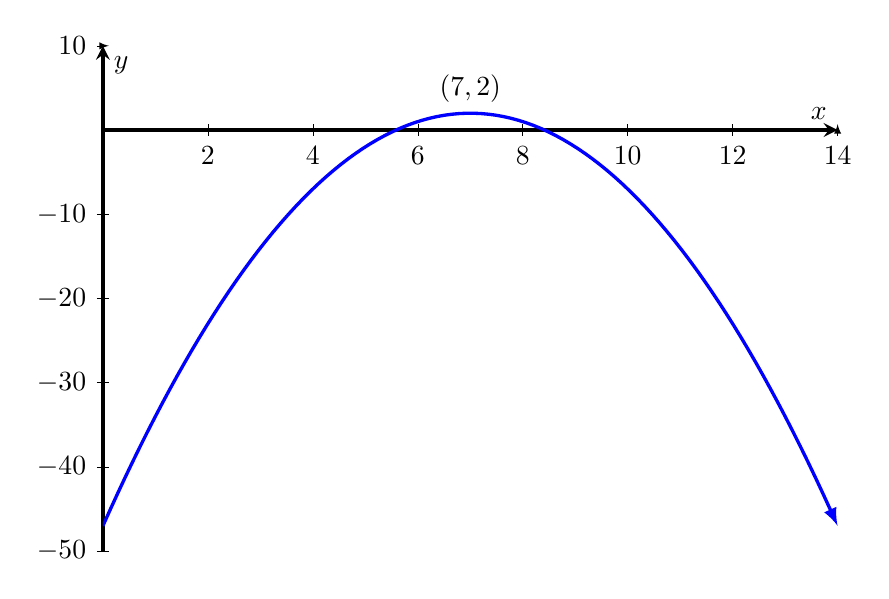
\begin{tikzpicture}
                \begin{axis}[
                    width=0.9\textwidth,
                    height=8cm,
                    axis lines = middle,
                    xlabel = $x$,
                    ylabel = $y$,
                    xmin=0, xmax=14,
                    ymin=-50, ymax=10,
                    tick style={black},
                    samples=100,
                    domain=0:14,
                ]
                
                    \addplot [blue, thick] {-(7-x)^2 + 2};
                    \node at (axis cs:7,2) [above] {\((7,2)\)};
                \end{axis}
            \end{tikzpicture}
            \caption{Wykres funkcji użytej do ewaluacji rozkładu godzin nauczycieli i klas na przestrzeni tygodnia.}
            \label{fig:funkcja_rownomiernosc}
        \end{figure}

        \subsubsection{Ocena względem nauczycieli}
            Dla każdego nauczyciela $t$ tworzony jest wektor dziennego obciążenia dydaktycznego $\boldsymbol{\beta}_t$.

            Zastosowanie funkcji $f(x)$ bez modyfikacji powodowałoby silne karanie dni wolnych ($x=0$), co jest niepożądane --- nauczyciel może mieć dzień wolny i nie powinno to stanowić wady planu.
            Aby temu zapobiec, zmodyfikowałem funkcję w następujący sposób:
            \[
                \begin{cases*}
                    f_T(x) = 0 & x = 0\\
                    f_T(x) = -\left(7-x\right)^2 + 2 & \text{ wpp.}\\
                \end{cases*}
            \]

            Ocena dla nauczyciela $t$ to suma wartości funkcji dla wszystkich dni tygodnia:
            \[ F_t = \sum_{d=1}^{5} f_T(\beta_{t,d}) \]

            Ocena wszystkich nauczycieli jest równa:
            \[ F_{T} = \sum_{t \in \mathcal{T}} F_t \]

        \subsubsection{Ocena względem klas}
            Proces jest analogiczny, przy czym dla klas dni wolne są niepożądane, więc nie stosuję dodatkowych modyfikacji funkcji.

            Oceny mają postać:
            \begin{align*}
                F_c &= \sum_{d=1}^{5} f(\beta_{c,d}) \\
                F_C &= \sum_{c \in \mathcal{C}} F_c
            \end{align*}

        \subsubsection{Normalizacja i wagi}
            Wyznaczanie końcowej wartości funkcji przystosowania wymaga uwzględnienia stosunku liczby nauczycieli do liczby uczniów.
            W typowych placówkach oświatowych liczba nauczycieli przywyższa liczbę klas.
            Bezpośrednie dodawanie ocen $F_T + F_C$ prowadziłoby do znaczącej dominacji oceny nauczycieli w ocenie końcowej.
            W celu rozwiązania tego problemu zastosowałem normalizację poprzez dzielenie każdej składowej przez odpowiednio $\left|\mathcal{T}\right|$ i $\left|\mathcal{C}\right|$.
            Takie podejście gwarantuje, że wpływ pojedynczej klasy na ocenę końcową jest porównywalny z wpływem pojedynczego nauczyciela.

            Kolejnym aspektem wymagającym uwzględnienia jest relatywna ważność obu kryteriów oceny. 
            W praktyce, wymagania równomiernego rozkładu dla każdej klasy są ważniejsze niż równomierny rozkład godzin nauczycieli.
            Aby umożliwić sterowanie tymi preferencjami należy zaimplementować wagi, co prowadzi do następującej postaci funkcji przystosowania dla $i$-tego osobnika:
            \[ F_i = \frac{\theta_T}{\left|\mathcal{T}\right|} F_{T,i} + \frac{\theta_C}{\left|\mathcal{C}\right|} F_{C,i}, \quad \theta_T, \theta_C \in \mathbb{R}^+ \]
            gdzie $\theta_T$ to waga oceny nauczycieli, a $\theta_C$ to waga oceny klas.

    \subsection{Selekcja}\label{subsection:selekcja}
        Zastosowałem tradycyjną metodę ruletkową. Polega ona na losowaniu osobników, którzy posłużą jako rodzice z prawdopodobieństwami, które sa proporcjonalne do wartości ich funkcji przystowania.
        Mając wektor ocen $F_{c\text{ total}} = \begin{bmatrix} F_1 & F_2 & \cdots & F_{\mathfrak{P}} \end{bmatrix}$, gdzie $\mathfrak{P}$ to rozmiar populacji, sortujemy go i dzielimy go na pół.
        Drugą połowę populacji, która ma najgorsze wyniki, usuwam i na jej miejsce wstawiam potomków rodziców wylosowanych zgodnie z prawdopodobieństwami:
        \[ P = \begin{bmatrix} \sigma\left(F_1\right) & \sigma\left(F_2\right) & \cdots & \sigma\left(F_{\frac{\mathfrak{P}}{2}}\right) \end{bmatrix}, \quad \sigma(F_i) = \frac{\exp\left[F_i\right]}{\sum_{j=1}^{\frac{\mathfrak{P}}{2}} \exp\left[F_j\right] } \]
        W celu zamiany funkcji przystosowania na prawdopodobieństwa użyłem funkcji SoftMax.

    \subsection{Krzyżowanie}\label{subsection:krzyzowanie}
        Największym wyzwaniem podczas projektowania algorytmu okazało się opracowanie krzyżowania osobników, które zagwarantowałoby spójność z nałożonymi ograniczeniami.
        Niemożność zaimplementowania takich rozwiązań jak proste modyfikowanie krzyżowania jednopunktowego zmusiło mnie do opracowania specjalistycznych metod.

        Z uwagi na dwie składowe funkcji przystosowania zdecydowałem się na zaimplementowanie dwóch niezależnych metod krzyżowania osobników widocznych w pseudokodach~\ref{alg:krzyzowanie_ocena_nauczyciel} oraz~\ref{alg:krzyzowanie_ocena_klasy}.
        Takie podejście umożliwia równoczesne dziedziczenie cech związanych z optymalnym obciążeniem dydaktycznym zarówno nauczycieli, jak i klas.
        Pozwala to także na stworzenie dwóch różnych potomków z dwóch rodziców.
        Wygenerowany w ten sposób osobniki $S'$ mają cechy, które gwarantują jak najlepsze przypisanie nauczycieli lub klas wśród obu rodziców.
        Następną zaletą tego podejścia jest fakt, że gwarantuje to też także spełnienie wszystkich wymagań,
        jako że wszystkie wymagania odnoszą się do indywidualnych bloków, a tych nie zmieniamy, tylko przepisujemy.

        \begin{algorithm}[H]
            \caption{Krzyżowanie uwzględniające ocenę obciążenia dydaktycznego nauczycieli}\label{alg:krzyzowanie_ocena_nauczyciel}

            \Input{$S_1$, $S_2$, oraz $F_{t,1}$, $F_{t,2}$ dla wszystkich nauczycieli $t\in\mathcal{T}$}
            \Output{Macierz potomka $S'$}
            
            $S' \gets \mathbf{0}_{5 \times \left|\mathcal{L}\right|}$ \;
            
            \For{$t \in \mathcal{T}$}{
                \Jesli{$F_{t,1} > F_{t,2}$}{
                    \For{\textnormal{każdego bloku} $L_i$ \textnormal{prowadzonego przez nauczyciela} $t$}{
                        \For{$d \in \{1,2,\dots,5\}$}{
                            $S'_{d,i} \gets S_{1,d,i}$ \;
                        }
                    }
                }
                \Wpp{
                    \For{\textnormal{każdego bloku} $L_i$ \textnormal{prowadzonego przez nauczyciela} $t$}{
                        \For{$d \in \{1,2,\dots,5\}$}{
                            $S'_{d,i} \gets S_{2,d,i}$ \;
                        }
                    }
                }
            }
            \Return $S'$
        \end{algorithm}
        \begin{algorithm}[H]
            \caption{Krzyżowanie uwzględniające ocenę obciążenia dydaktycznego klas}\label{alg:krzyzowanie_ocena_klas}

            \Input{$S_1$, $S_2$, oraz $F_{c,1}$, $F_{c,2}$ dla wszystkich klas $c\in\mathcal{C}$}
            \Output{Macierz potomka $S'$}
            
            $S' \gets \mathbf{0}_{5 \times \left|\mathcal{L}\right|}$ \;
            
            \For{$t \in \mathcal{T}$}{
                \Jesli{$F_{c,1} > F_{c,2}$}{
                    \For{\textnormal{każdego bloku} $L_i$ \textnormal{dla klasy} $c$}{
                        \For{$d \in \{1,2,\dots,5\}$}{
                            $S'_{d,i} \gets S_{1,d,i}$ \;
                        }
                    }
                }
                \Wpp{
                    \For{\textnormal{każdego bloku} $L_i$ \textnormal{prowadzonego przez nauczyciela} $t$}{
                        \For{$d \in \{1,2,\dots,5\}$}{
                            $S'_{d,i} \gets S_{2,d,i}$ \;
                        }
                    }
                }
            }
            \Return $S'$
        \end{algorithm}
            % Funkcja krzyżowania uwzględniająca ocenę rozkładu godzin nauczycieli definiuje się następująco:

            % \noindent
            % \textbf{Dane wejściowe:}
            %     \begin{itemize}
            %         \item $S_1$ --- pierwszy rodzic,
            %         \item $S_2$ --- drugi rodzic,
            %         \item $F_{t,1}$ --- ocena wszystkich nauczycieli $t \in \mathcal{T}$ pierwszego osobnika,
            %         \item $F_{t,2}$ --- ocena wszystkich nauczycieli $t \in \mathcal{T}$ drugiego osobnika.
            %     \end{itemize}
            
            % \noindent
            % \textbf{Działanie:}
            % \begin{enumerate}
            %     \item Inicjalizacja macierzy potomka: $S'} = \mathbf{0}_{5 \times \left|\mathcal{L}\right|}$
            %     \item Dla każdego nauczyciela $t \in \mathcal{T}$:
            %     \begin{enumerate}
            %         \item Jeśli $F_{t,1} > F_{t,2}$, przepisz wszystkie kolumny odpowiadające blokom prowadzonym przez nauczyciela $t$ z macierzy $S_1$ do $S'}$.
            %         \item W przeciwnym przypadku, przepisz kolumny z macierzy $S_2$.
            %     \end{enumerate}
            % \end{enumerate}

            % Wygenerowany w ten sposób osobnik $S'$ ma cechy, które gwarantują jak najlepsze przypisanie nauczycieli wśród obu rodziców.
            % Następną zaletą tego podejścia jest fakt, że gwarantuje to też także spełnienie wszystkich wymagań,
            % jako że wszystkie wymagania odnoszą się do indywidualnych bloków, a tych nie zmieniamy, tylko przepisujemy.

        % \subsubsection{Względem oceny klas}
        %     Analogicznie definiujemy krzyżowanie względem oceny klas:

        %     \noindent
        %     \textbf{Dane wejściowe:}
        %         \begin{itemize}
        %             \item $S_1$ --- pierwszy rodzic,
        %             \item $S_2$ --- drugi rodzic,
        %             \item $F_{c,1}$ --- ocena wszystkich klas $c \in \mathcal{C}$ pierwszego osobnika,
        %             \item $F_{c,2}$ --- ocena wszystkich klas $c \in \mathcal{C}$ drugiego osobnika.
        %         \end{itemize}
            
        %     \noindent
        %     \textbf{Działanie:}
        %     \begin{enumerate}
        %         \item Inicjalizacja macierzy potomka: $S' = \mathbf{0}_{5 \times \left|\mathcal{L}\right|}$
        %         \item Dla każdej klasy $c \in \mathcal{C}$:
        %         \begin{enumerate}
        %             \item Jeśli $F_{c,1} > F_{c,2}$, przepisz wszystkie kolumny odpowiadające blokom klasy $c$ z macierzy $S_1$ do $S'$.
        %             \item W przeciwnym przypadku przepisz kolumny z macierzy $S_2$.
        %         \end{enumerate}
        %     \end{enumerate}

            % Wygenerowany w ten sposób osobnik $S'$ ma cechy, które gwarantują jak najlepszy rozkład godzin lekcyjnych dla klas wśród obu rodziców.
            % Podobnie w tym przypadku nie modyfikujemy przydziału godzin w indywidualnych blokach, więc zachowujemy zgodność z ograniczeniami.

    \subsection{Mutacja}\label{subsection:mutacja}
        Analogicznie do przypadku krzyżowania, zastosowanie prostych metod mutacji (takich jak losowa zamiana pojedynczych przydziałów) nie jest możliwe ze względu na wysokie ryzyko naruszenia ograniczeń.
        W szczególności, modyfikacja pojedynczych wartości macierzy $S$ może prowadzić do niezgodności z warunkiem głównym bloków.
        
        W odpowiedzi na to wyzwanie, przyjąłem strategię mutacji operującą na poziomie bloków --- kolumn macierzy przydziałów, podobną do podejścia zastosowanego w funkcji krzyżowania.
        Pozwana to na zachowania zgodności z ograniczeniami.
        
        \begin{samepage}
            Procedura mutacji definiuje się następująco:
            \begin{enumerate}
                \item Z populacji wybieranych jest losowo $n$ osobników.
                \item Dla każdego wybranego osobnika wybierany jest losowy podzbiór kolumn (bloków lekcyjnych).
                \item Dla każdej wybranej kolumny $j$ wylosuj nowy przydział zgodnie z procedurą opisaną w podrozdziale~\ref{subsection:generowanie_populacji}.
            \end{enumerate}
        \end{samepage}
        
        Takie podejście gwarantuje, że zmutowane osobniki zachowują zgodność z podstawowymi ograniczeniami problemu, jednocześnie wprowadzając do populacji nowe warianty rozkładów godzinowych wybranych bloków lekcyjnych.

        W celu zwiększenia stabilności procesu ewolucyjnego zaimplementowałem także elitarnego osobnika, który zawsze pojawia się niezmieniony w następnej generacji.
        Jest to osobik o największej wartości funkcji przystosowania:
        \[ S_{\text{best}} = S_i, \quad i = \underset{j \in \left\{1, 2, \dots \mathfrak{P}\right\}}{\arg\max} F_j \]

    \subsection{Przykładowy wynik}
        Dla danych wejściowych przedstawionych w poprzednim przykładzie algorytm wygenerował następującego najlepszego osobnika:
        \[ S_{\text{best}} = \begin{bmatrix}
            1 & \cdots & 0 & \cdots & 0 & \cdots \\
            0 & \cdots & 1 & \cdots & 0 & \cdots \\
            0 & \cdots & 0 & \cdots & 1 & \cdots \\
            0 & \cdots & 0 & \cdots & 0 & \cdots \\
            1 & \cdots & 0 & \cdots & 0 & \cdots 
        \end{bmatrix} \]
        Interpretacja macierzy przydziału jest następująca:
        \begin{itemize}
            \item blok językowy (niemiecki + francuski + rosyjski) został umieszczony po jednej godzinie w poniedziałek oraz piątek,
            \item jedna godzina wspólnego bloku informatyki i języka angielskiego została przydzielona do wtorku,
            \item jedna godzina chemii została przypisana do środy.
        \end{itemize}

        Na rysunku~\ref{fig:wyniki_ewolucyjny} przedstawiłem wartości funkcji celu dla pięciu niezależnych uruchomień algorytmu genetycznego dla 25 generacji, przy następujących parametrach:
        \begin{itemize}
            \item $\mathfrak{P} = 1000$,
            \item $\theta_T = 1$,
            \item $\theta_G = 2$.
        \end{itemize}

        \begin{figure}[H]
            \centering
            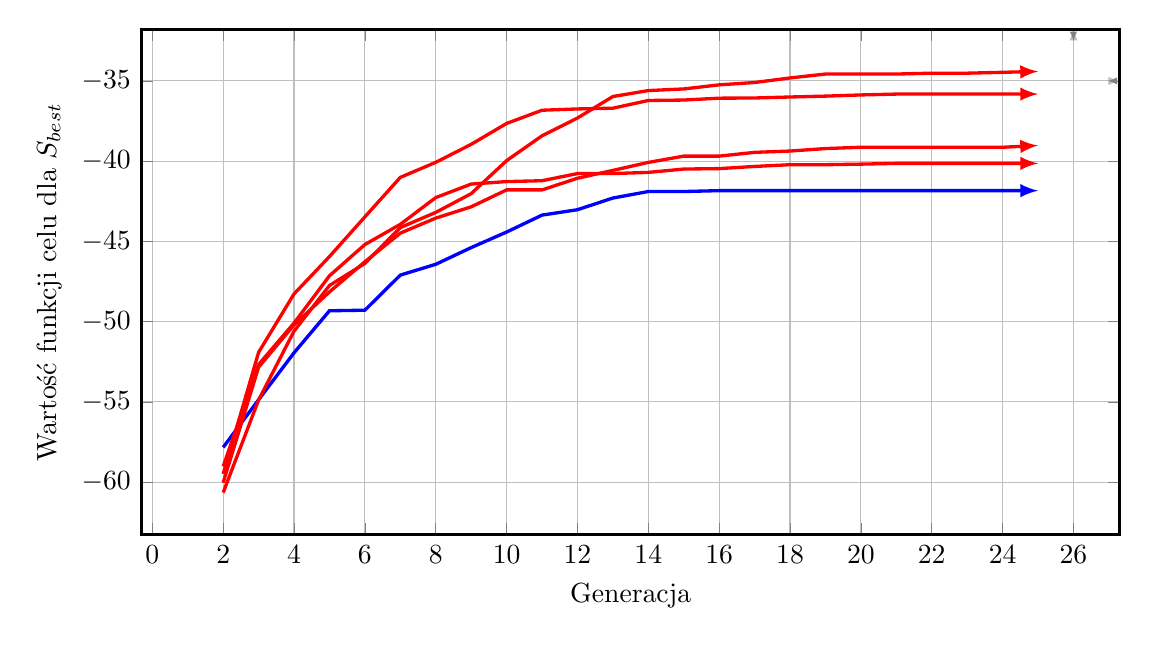
\begin{tikzpicture}
                \begin{axis}[
                    width=14cm,
                    height=8cm,
                    xlabel={Generacja},
                    ylabel={Wartość funkcji celu dla $S_{\text{best}}$},
                    grid=both,
                    legend style={at={(1.02,1)}, anchor=north west},
                    each nth point={1}, % rysuje wszystkie punkty
                ]
                
                % --- Linia 1 ---
                \addplot[
                    thick,
                    blue,
                ] table[row sep=\\] {
                    x y
                    1 -70.54422604422604 \\
                    2 -57.83538083538084 \\
                    3 -54.86855036855037 \\
                    4 -51.94226044226045 \\
                    5 -49.32432432432432 \\
                    6 -49.287469287469285 \\
                    7 -47.1007371007371 \\
                    8 -46.42628992628993 \\
                    9 -45.38697788697789 \\
                    10 -44.41769041769042 \\
                    11 -43.36240786240786 \\
                    12 -43.02579852579852 \\
                    13 -42.298525798525795 \\
                    14 -41.891891891891895 \\
                    15 -41.891891891891895 \\
                    16 -41.83783783783784 \\
                    17 -41.83783783783784 \\
                    18 -41.83783783783784 \\
                    19 -41.83783783783784 \\
                    20 -41.83783783783784 \\
                    21 -41.83783783783784 \\
                    22 -41.83783783783784 \\
                    23 -41.83783783783784 \\
                    24 -41.83783783783784 \\
                    25 -41.83783783783784 \\
                };
                
                % --- Linia 2 ---
                \addplot[
                    thick,
                    red,
                ] table[row sep=\\] {
                    x y
                    1 -72.02211302211302 \\
                    2 -59.024570024570025 \\
                    3 -52.671990171990174 \\
                    4 -50.08968058968058 \\
                    5 -47.14496314496314 \\
                    6 -45.195331695331696 \\
                    7 -43.937346437346434 \\
                    8 -42.270270270270274 \\
                    9 -41.42751842751842 \\
                    10 -41.27272727272727 \\
                    11 -41.21867321867321 \\
                    12 -40.77272727272727 \\
                    13 -40.77272727272727 \\
                    14 -40.7002457002457 \\
                    15 -40.4914004914005 \\
                    16 -40.464373464373466 \\
                    17 -40.32923832923833 \\
                    18 -40.221130221130224 \\
                    19 -40.221130221130224 \\
                    20 -40.18550368550369 \\
                    21 -40.13882063882063 \\
                    22 -40.13882063882063 \\
                    23 -40.13882063882063 \\
                    24 -40.13882063882063 \\
                    25 -40.13882063882063 \\
                };

                \addplot[
                    thick,
                    red,
                ] table[row sep=\\] {
                    x y
                    1 -74.76781326781327 \\
                    2 -59.492628992628994 \\
                    3 -51.91523341523341 \\
                    4 -48.27395577395577 \\
                    5 -45.94594594594595 \\
                    6 -43.47174447174448 \\
                    7 -41.01105651105651 \\
                    8 -40.073710073710075 \\
                    9 -38.95208845208845 \\
                    10 -37.64987714987715 \\
                    11 -36.82678132678133 \\
                    12 -36.74570024570025 \\
                    13 -36.699017199017206 \\
                    14 -36.218673218673224 \\
                    15 -36.19164619164619 \\
                    16 -36.07493857493858 \\
                    17 -36.06388206388207 \\
                    18 -36.001228501228496 \\
                    19 -35.94717444717444 \\
                    20 -35.87346437346437 \\
                    21 -35.81941031941032 \\
                    22 -35.81941031941032 \\
                    23 -35.81941031941032 \\
                    24 -35.81941031941032 \\
                    25 -35.81941031941032 \\
                };

                \addplot[
                    thick,
                    red,
                ] table[row sep=\\] {
                    x y
                    1 -73.96560196560198 \\
                    2 -60.654791154791155 \\
                    3 -54.882063882063875 \\
                    4 -50.59582309582309 \\
                    5 -47.749385749385745 \\
                    6 -46.37469287469287 \\
                    7 -44.13882063882063 \\
                    8 -43.19410319410319 \\
                    9 -42.02579852579852 \\
                    10 -39.966830466830466 \\
                    11 -38.42014742014743 \\
                    12 -37.31203931203931 \\
                    13 -35.971744471744465 \\
                    14 -35.6007371007371 \\
                    15 -35.5 \\
                    16 -35.24447174447174 \\
                    17 -35.09828009828009 \\
                    18 -34.81449631449631 \\
                    19 -34.57125307125307 \\
                    20 -34.57125307125307 \\
                    21 -34.57125307125307 \\
                    22 -34.51719901719902 \\
                    23 -34.51719901719902 \\
                    24 -34.46314496314496 \\
                    25 -34.40909090909091 \\
                };

                \addplot[
                    thick,
                    red,
                ] table[row sep=\\] {
                    x y
                    1 -73.21990171990171 \\
                    2 -60.035626535626534 \\
                    3 -52.83660933660933 \\
                    4 -50.20761670761671 \\
                    5 -48.148648648648646 \\
                    6 -46.26904176904176 \\
                    7 -44.486486486486484 \\
                    8 -43.550368550368546 \\
                    9 -42.845208845208845 \\
                    10 -41.79115479115479 \\
                    11 -41.79115479115479 \\
                    12 -41.065110565110565 \\
                    13 -40.576167076167074 \\
                    14 -40.07739557739558 \\
                    15 -39.68673218673219 \\
                    16 -39.68673218673219 \\
                    17 -39.45085995085996 \\
                    18 -39.36977886977887 \\
                    19 -39.214987714987714 \\
                    20 -39.13390663390663 \\
                    21 -39.13390663390663 \\
                    22 -39.13390663390663 \\
                    23 -39.13390663390663 \\
                    24 -39.13390663390663 \\
                    25 -39.02579852579852 \\
                };
                
                \end{axis}
            \end{tikzpicture}
            \caption{Wykres wartości funkcji cely dla pięciu uruchomień algorytmu genetycznego}\label{fig:wyniki_ewolucyjny}
        \end{figure}
        Średni czas obliczeń dla pięciu prób wyniósł 95.88 s.  
        W żadnym przypadku funkcja celu nie osiągnęła wartości dodatnich.
        Wynika to z faktu, że w danych wejściowych występują klasy oraz nauczyciele, którzy mają liczbę bloków znacząco mniejszą niż 35.
        W praktyce uniemożliwia to uzyskiwanie dodatnich wartości funkcji celu, ponieważ algorytm nie ma wystarczającej liczby bloków, by spełnić wszystkie wymagania strukturalne konieczne do uzyskania pozytywnego wyniku.

\section{Solver programowania liniowego z ograniczeniami}\label{section:solver}
    W trzecim etapie algorytmu wykorzystuję solver programowania liniowego z ograniczeniami (Constraint Programming --- CP).
    W odróżnieniu od czystego programowania liniowego (MIP), solver CP operuje na szerszej klasie ograniczeń, w tym na zmiennych interwałowych, co czyni go idealnym narzędziem do problemów harmonogramowania.
    W odpowiedzi na wyzwania napotkane w podejściu opisanym w podrozdziale~\ref{subsection:podejscie_zerojedynkowe} zdecydowałem się na wykorzystanie zmiennych interwałowych opisanych dokładniej w dokumentacji OR-Tools~\cite{googleortoolsintervalvar}. 

    Zalety podejścia CP:
        \begin{itemize}
            \item \textbf{Naturalne modelowanie}: Zmienne interwałowe bezpośrednio reprezentują zajęcia o określonym czasie rozpoczęcia i zakończenia.
            \item \textbf{Efektywność pamięciowa}: W porównaniu z reprezentacją binarną z podrozdziału~\ref{subsection:podejscie_zerojedynkowe}, podejście interwałowe redukuje liczbę zmiennych decyzyjnych.
            \item \textbf{Specjalizowane ograniczenia}: Solver oferuje gotowe implementacje ograniczeń typowych dla harmonogramów --- nakładanie się interwałów.
        \end{itemize}

    Proces jest wykonywany niezależnie dla każdego dnia tygodnia $d \in \{1,2,3,4,5\}$, reprezentowanego przez wiersze macierzy $S_{\text{best}}$.
    Dla każdego dnia rozwiązujemy podproblem zawierający tylko te bloki $L_i$, dla których $S_{\text{best}_{d,i}}> 0$. \\
    Takie podejście:
    \begin{itemize}
        \item Redukuje wymagania pamięciowe o $\approx 5$.
        \item Umożliwia równoległe przetwarzanie dni, jeśli nie ogranicza nas pamięć.
        \item Upraszcza strukturę ograniczeń.
    \end{itemize}

    \subsection{Reprezentacja interwałów}
        Dla modelowania zajęć używamy zmiennych interwałowych, które reprezentują bloki czasowe o określonej długości:
        \begin{itemize}
            \item \textbf{Interwał podstawowy} dla bloku lekcyjnego $L_i \in \mathcal{L}$:
                \[  I_i = (s_i, v_i, e_i):
                    \begin{cases}
                        s_i &\in \left[0, H\right] \\
                        d_i &= v_i \\
                        e_i &\in \left[0, H\right] \\
                        e_i &= s_i + d_i    
                    \end{cases}
                \]
                gdzie $s_i$ to czas rozpoczęcia, $e_i$ to czas zakończenia, a $d_i$ to czas trwania.
            
            \item \textbf{Interwał opcjonalny} dla przypisania sali:
                \[ O_{i,t,r} =
                    \begin{cases}
                        p_{i,j,r} &\in \left\{0, 1\right\}\\
                        p_{i,j,r} &\implies e_i = s_i + d_i
                    \end{cases}
                \]
        \end{itemize}

    \subsection{Zmienne decyzyjne}
        \subsubsection{Interwały bloków lekcyjnych}
            Dla każdego bloku $L_i \in \mathcal{L}$ z liczbą godzin $v_i > 0$ definiujemy:
            \[ I_i = (s_i, v_i, e_i) \]

        \subsubsection{Przypisania sal}
            Dla każdej możliwej kombinacji (blok, nauczyciel, sala) definiujemy interwał opcjonalny:
            \[ O_{L_i,t,r} = (s_i, v_i, e_i, p_{L_i,t,r}), \quad \begin{cases}
                L_i &\in \mathcal{L} \\
                t &\in \mathcal{T} \\
                r &\in \mathcal{R}
            \end{cases} \]
            gdzie brane pod uwagę są tylko mozliwe kombinacje. Przykładowo blok lekcyjny z jednym wymaganiem głównym matematyki, nauczyciel matematyki oraz sala do matematyki.

    \subsection{Ograniczenia}
        \subsubsection{Ograniczenie przypisania sal}
            Dla każdego bloku $L_i$ musi być przypisana odpowiednia liczba sal:
            \[ \forall L_i \in \mathcal{L}: \sum_{r \in \mathcal{R}, t \in \mathcal{T}} p_{L_i,t,r} = |T_i| \]

        \subsubsection{Ciągłość zajęć dla klas}
            Dla każdej klasy $c \in \mathcal{C}$ i dnia $d \in \{1, 2, \dots,5\}$:
            \[ \mathcal{L}_{c,d} = \{L_i \in \mathcal{L}: \exists w \in L_i \text{ takie, że } c_w = c \land s_{\text{best}_{d,i}} > 0\} \]
            \textbf{Nienakładanie się zajęć}~\cite{googleortoolsoverlap}\textbf{:}
            \[ \text{AddNoOverlap}(\{I_i : L_i \in \mathcal{L}_{c,d}\}) \]
            \textbf{Brak okienek:}
            \[
                \begin{cases}
                    \text{start}_c = \min\{s_i : L_i \in \mathcal{L}_{c,d}\} \\
                    \text{end}_c = \max\{e_i : L_i \in \mathcal{L}_{c,d}\} \\
                    \text{end}_c - \text{start}_c = \sum_{L_i \in \mathcal{L}_{c,d}} v_i
                \end{cases}
            \]

        \subsubsection{Nakładanie się nauczycieli}
            Dla każdego nauczyciela $t \in \mathcal{T}$ i dnia $d \in \{1, 2, \dots,5\}$:
            \[ \mathcal{L}_{t,d} = \{L_i \in \mathcal{L}: t \in T_i \land s_{\text{best}_{d,i}} > 0\} \]
            \[ \text{AddNoOverlap}(\{I_i : L_i \in \mathcal{L}_{t,d}\}) \]

        \subsubsection{Kolizje sal}
            Dla każdej sali $r \in \mathcal{R}$ i dnia $d \in \{1, 2, \dots,5\}$:
            \[ \mathcal{O}_{r,d} = \{O_{L_i,t,r} : L_i \in \mathcal{L}, t \in \mathcal{T}, s_{\text{best}_{d,i}} > 0\} \]
            \[ \text{AddNoOverlap}(\mathcal{O}_{r,d}) \]
        
        \subsubsection{Sekwencjonowanie przedmiotów}
            Ograniczenie dotyczące dwuch takich samych przedmiotów jednego dnia jest łatwo rozwiązywane poprzez zastosowanie interwałów, gdyż z definicji mamy zagwarantowane, że:
            \[ \forall i \in \left\{1, 2, \dots, \left|\mathcal{L}\right|\right\}: v_i = 2 \implies e_i - s_i = 2 \]
            W ten sposób jeśli do danego dnia są przypisane dwie godziny $i$-tego bloku, to mamy gwarancję, że następują one po sobie.

    \subsection{Funkcja celu}
        Minimalizujemy całkowity czas przebywania nauczycieli w szkole:
        \[
            \forall t \in \mathcal{T}, d \in \{1,2,\dots,5\}:
            \begin{cases}
                \text{start}_{t,d} &= \min\{s_i : L_i \in \mathcal{L}_{t,d}\} \\
                \text{end}_{t,d} &= \max\{e_i : L_i \in \mathcal{L}_{t,d}\} \\
                \text{duration}_{t,d} &= \text{end}_{t,d} - \text{start}_{t,d}
            \end{cases}
        \]

        \[ F = \sum_{t \in \mathcal{T}} \sum_{d=1}^{5} \text{duration}_{t,d} \]

        Minimalizacja tej funkcji prowadzi do kompaktowego układania zajęć, redukując okienka w planach nauczycieli.

    \subsection{Transformacja interwałów na przypisania końcowe}
        Po znalezieniu rozwiązania przez solver CP-SAT, konieczne jest przekształcenie zmiennych interwałowych na ostateczne przypisania w zbiorze $\mathcal{Z}$.
        Proces ten obejmuje ekstrakcję wartości zmiennych decyzyjnych i mapowanie na strukturę danych planu lekcji.
        
        \subsubsection{Ekstrakcja rozwiązań z solvera}
            Dla każdego interwału $I_i$ w rozwiązaniu zapisujemy następujące wartości:
            \begin{itemize}
                \item $L_i$
                \item $s_i$
                \item $e_i$
                \item $v_i$
                \item $d$ --- aktualnie przetwarzany dzień tygodnia
                \item $\mathcal{R}_i = \left\{r \in \mathcal{R}: \exists t \in \mathcal{T} \text{ takie, że } p_{i,t,r} = 1 \right\}$ --- zbiór aktywnych sal, które zostały przypisane do bloku $L_i$.
            \end{itemize}
        
        \subsubsection{Mapowanie na strukturę lekcji}
            Dla każdych takich wartości tworzymy konkretne lekcje w zbiorze $\mathcal{Z}$.
            Wpierw tworzymy funkcję, która będzie przypisywać nauczycieli i prowadzone przez nich przedmioty $s$ do odpowiednich sal.
            \begin{align*}
                f: T_i &\to \mathcal{R}_i \\
                \forall t \in T_i: f(t) &= r \in \mathcal{R}_i \text{ takie, że } r \text{ obsługuje przedmiot } s \in \vec{S}_{L_i}
            \end{align*}
            Konieczne jest użycie takiej funkcji, ponieważ każdy nauczyciel w jednym bloku może mieć przypisane wiele klas.
            Musimy stworzyć wiele przypisań, które będą miały taką samą salę $r$ dla każdej klasy.

            Dla każdego wymagania $w \in L_i$ i każdego slotu czasowego $h \in \left[1, e_i-s_i\right]$:
            \begin{align*}
                z &= (d, h, c_w, t_w, s_w, f(t_w)) \\
                \mathcal{Z}_d &\gets \mathcal{Z}_d \cup \{z\}
            \end{align*}
        
        \subsubsection{Przykład transformacji}
            Rozważmy blok $L_i = \{w_1, w_2\}$ z $v_i = 2$, gdzie:
            \begin{itemize}
                \item $w_1 = (t_1, c_1, s_1, 3)$ --- nauczyciel $t_1$, klasa $c_1$, wychowanie fizyczne
                \item $w_2 = (t_2, c_1, s_2, 3)$ --- nauczyciel $t_2$, klasa $c_1$, wychowanie fizyczne
            \end{itemize}
            
            Po rozwiązaniu otrzymujemy przypisania:
            \begin{align*}
                z_1 &= (1, 2, c_A, t_1, s_1, r_1) \\
                z_2 &= (1, 3, c_A, t_1, s_1, r_1) \\
                z_3 &= (1, 2, c_A, t_2, s_2, r_2) \\
                z_4 &= (1, 3, c_A, t_2, s_2, r_2)
            \end{align*}

            Jest to równoznaczne z leckją wychowania fizycznego podzieloną na dwie grupy, które odbywają się w tym samym czasie.

        Proces ten powtarzamy dla wszystkich dni tygodnia, tworząc kompletny plan lekcji $\mathcal{Z} = \bigcup_{d=1}^5 \mathcal{Z}_d$ spełniający wszystkie ograniczenia i optymalizujący funkcję celu.

    \subsection{Przykładowy wynik}
        Dla danych wejściowych przedstawionych w poprzednim przykładzie mamy następujące przypisania:
        \[
            \mathcal{Z} = \left\{ 
                \begin{aligned}
                    &\left(1, 3, \text{IVA}, \text{Jn1}, \text{J.Niem}, 11\right), \\
                    &\left(1, 3, \text{IVF}, \text{Jn1}, \text{J.Niem}, 11\right), \\
                    &\left(1, 3, \text{IVA}, \text{Jr1}, \text{J.Ros}, 19\right), \\
                    &\left(1, 3, \text{IVG}, \text{Jr1}, \text{J.Ros}, 19\right), \\
                    &\left(1, 3, \text{IVD}, \text{Jf2}, \text{J.Fran}, 20\right), \\
                    &\left(1, 3, \text{IVF}, \text{Jf2}, \text{J.Fran}, 20\right), \\
                    &\vdots \\
                    &\left(2, 7, \text{IA}, \text{Ja5}, \text{J.Ang}, 9\right) \\
                    &\left(2, 7, \text{IA}, \text{Inf2}, \text{Informatyka}, \text{Sala Informatyczna 2}\right), \\
                    &\vdots \\
                    &\left(3, 7, \text{IG}, \text{Chem1}, \text{Chemia}, \text{Sala do Chemii 1}\right)          
                \end{aligned}
            \right\}
        \]